\documentclass[11pt,letterpaper]{article}

% ---------------------------------------------------------------------------
% Structural autocatalysis can be common while productive operation is rare:
% an exact separation theorem in a capped-Zipf binary polymer model.
%
% Author metadata: set the macros below before submission.  The companion
% critical-window manuscript is cited through \CompanionAuthor.
% ---------------------------------------------------------------------------
\newcommand{\PaperAuthor}{Author name to be inserted}
\newcommand{\PaperAffiliation}{Affiliation to be inserted}
\newcommand{\PaperDate}{13 September 2026}
\newcommand{\CompanionAuthor}{Author name to be inserted}

\usepackage[T1]{fontenc}
\usepackage[utf8]{inputenc}
\usepackage{lmodern}
\usepackage{microtype}
\usepackage[letterpaper,margin=1in]{geometry}
\usepackage{amsmath,amssymb,amsthm,mathtools}
\usepackage{booktabs,array,longtable}
\usepackage{graphicx}
\usepackage{enumitem}
\usepackage{xcolor}
\usepackage{tikz}
\usetikzlibrary{arrows.meta,positioning,calc}
\usepackage[numbers,sort&compress]{natbib}
\usepackage[colorlinks=true,linkcolor=blue!50!black,citecolor=blue!50!black,urlcolor=blue!50!black]{hyperref}
\hypersetup{pdftitle={Structural autocatalysis can be common while productive operation is rare},
  pdfkeywords={autocatalytic sets, RAF, binary polymer model, power-law catalysis, stochastic mass action, critical window, Lean 4}}

%% Breakable typewriter identifiers for Lean names: \lean{Foo.bar_baz}
\makeatletter
\let\lean@us=_
\let\lean@end\relax
\DeclareRobustCommand{\lean}[1]{\begingroup\ttfamily\lean@scan#1\lean@end}
\def\lean@scan#1{\ifx#1\lean@end\endgroup\else\lean@char{#1}\expandafter\lean@scan\fi}
\def\lean@char#1{\ifx#1\lean@us\char`\_\allowbreak\else\ifx#1.\char`\.\allowbreak\else#1\fi\fi}
\makeatother

\setlist{itemsep=2pt,topsep=3pt}
\setlength{\emergencystretch}{2em}

\theoremstyle{plain}
\newtheorem{theorem}{Theorem}[section]
\newtheorem{proposition}[theorem]{Proposition}
\newtheorem{lemma}[theorem]{Lemma}
\newtheorem{corollary}[theorem]{Corollary}
\theoremstyle{definition}
\newtheorem{definition}[theorem]{Definition}
\theoremstyle{remark}
\newtheorem{remark}[theorem]{Remark}
\numberwithin{equation}{section}

\newcommand{\PP}{\mathbb P}
\newcommand{\EE}{\mathbb E}
\newcommand{\QQ}{\mathbb Q}
\newcommand{\R}{\mathbb R}
\newcommand{\N}{\mathbb N}
\newcommand{\XX}{\mathcal X}
\newcommand{\RR}{\mathcal R}
\newcommand{\cF}{\mathcal F}
\newcommand{\cS}{\mathcal S}
\newcommand{\cC}{\mathcal C}
\newcommand{\cG}{\mathcal G}
\newcommand{\eps}{\varepsilon}
\newcommand{\ind}{\mathbf 1}
\newcommand{\cl}{\operatorname{cl}}
\newcommand{\dd}{\,\mathrm dt}
\newcommand{\thetaq}{\theta(q_*)}
\newcommand{\cat}{\mathrm{cat}}
\newcommand{\bas}{\mathrm{basal}}
\newcommand{\Bcoef}{B}
\newcommand{\Dp}{D}

\title{Structural autocatalysis can be common\\ while productive operation is rare:\\
\large an exact separation theorem in a capped-Zipf binary polymer model}
\author{\PaperAuthor\\[2pt]\small\PaperAffiliation}
\date{\PaperDate}

\begin{document}
\maketitle

\begin{abstract}
A reflexively autocatalytic and food-generated reaction set (RAF) certifies that a reaction network is closed under the resources and catalysts it needs. It does not say whether a reactor started from food alone will actually produce material. We compare the two questions in one explicit random model: the reversible binary polymer model with molecules of length at most $n$, food consisting of the monomers and dimers, and the capped-Zipf catalysis law of Hordijk and Steel at the critical exponent sequence $a_n=2-2/n$, under which each molecule catalyzes on average $9n/\pi^2$ reactions. Three statements are proved for the same sampled network. First, the probability that a RAF exists converges to $\theta(q_*)\in(0,1)$, the survival probability of an infinite independent reversible reaction-closure process at openness $q_*=1-e^{-9/\pi^2}$. Second, conditional on existence, the minimum RAF size $M_n$ satisfies $\log M_n/n\to0$ in probability, with an explicit subexponential cutoff attaining the full limiting mass. Third, in a fed, diluted stochastic mass-action reactor with all spontaneous reactions active, the probability that the reactor keeps its total mass bounded and exports a fixed positive amount of nonfood polymer during a fixed observation window is bounded above and below by constant multiples of the single-incidence probability $p_n\sim9/(\pi^2X_n)$, where $X_n=2^{n+1}-2$ is the number of molecular species, up to an explicit molecular-noise error that a sufficient quadratic volume scale makes negligible. The same order holds jointly with, and conditionally on, the existence of some RAF, and the same conclusions hold for the fraction of catalytic environments in which a reactor run succeeds with high probability. Removing catalysis makes the same output observable asymptotically negligible. Thus structural autocatalysis occurs with probability bounded away from zero and small structural certificates are typical, while the specified productive operation has probability of order $1/X_n$, decaying exponentially in $n$. The structural limits, the finite probability sandwich, and their asymptotic corollaries are formally verified in Lean~4; the remaining steps are conventional proofs given in full.
\end{abstract}

\section{Introduction}\label{sec:intro}

Collectively autocatalytic sets were proposed by Kauffman \cite{kauffman1986autocatalytic} as a route by which a random chemistry could bootstrap a self-sustaining organization without a single self-replicating molecule. Their combinatorial formalization is the notion of a reflexively autocatalytic and food-generated set, or RAF, introduced by Steel \cite{steel2000emergence} and developed with Hordijk \cite{hordijk2004detecting,steel2019autocatalytic}: a nonempty set of reactions that can generate every molecule it needs from an ambient food set, and whose every reaction has a catalyst among the molecules generated. In the binary polymer model \cite{kauffman1986autocatalytic,steel2000emergence,hordijk2004detecting}, where molecules are binary strings and reactions are ligations and cleavages, RAFs appear once the mean number of reactions catalyzed per molecule grows linearly in the maximum string length $n$ \cite{mossel2005random,hordijk2011required}. Hordijk and Steel \cite{hordijk2016variable} showed that the distribution of catalytic activity across molecules affects both the appearance and the size of RAFs, and singled out power-law (capped Zipf) catalysis as a natural heterogeneous alternative to uniform catalysis.

A RAF is a statement about closure. It says nothing by itself about waiting times, competition between reactions, dilution, or the amount of material that a reactor actually exports; this gap between structural and dynamical autocatalysis has been discussed since the first kinetic simulations of the model \cite{farmer1986autocatalytic} and is central to critiques of metabolism-first scenarios \cite{vasas2010lack,hordijk2014evolvability}. This paper quantifies the gap for one fully specified random model. We fix the capped-Zipf sampler at the critical sequence $a_n=2-2/n$, place the sampled network in a fed, diluted, well-mixed stochastic mass-action reactor whose only initial molecules are food, and measure a deliberately physical event: total polymer mass stays bounded and a fixed positive amount of nonfood polymer is exported during a fixed time window. Under one probability space that samples the catalytic environment, the kinetic coefficients, and the reactor trajectory, we prove the following.

\begin{itemize}
\item \textbf{Structural existence.} The probability that a RAF exists converges to $\thetaq$, a number strictly between $0$ and $1$ (Theorem~\ref{thm:main}(i)).
\item \textbf{Structural size.} Conditional on existence, the minimum RAF has subexponential size: for every $b>0$, $\PP(M_n\le2^{bn}\mid\text{RAF exists})\to1$, and one explicit stretched-exponential cutoff captures the whole limiting mass (Theorem~\ref{thm:main}(ii)).
\item \textbf{Productive rarity.} At a sufficient quadratic volume scale, the probability of the productive event is $\Theta(p_n)=\Theta(1/X_n)$, where $p_n$ is the probability that a fixed molecule catalyzes a fixed reaction and $X_n=2^{n+1}-2$ is the number of species; the same order holds jointly with, and conditionally on, RAF existence, and also for the fraction of catalytic environments in which a reactor run succeeds with high probability (Theorem~\ref{thm:main}(iii) and Corollary~\ref{cor:environment}). With catalysis switched off, the same observable has probability $o(p_n)$ (Theorem~\ref{thm:main}(iv)).
\end{itemize}

So the structural certificate is common and typically small, while the productive requirement is exponentially rare in $n$, in the same sampled network and after conditioning on the certificate. The theorem is an asymptotic probability statement with explicit but very conservative constants; it is not a calibrated prediction of a transition, and it does not say that RAFs are chemically inactive. Section~\ref{sec:discussion} states precisely what is and is not implied.

\paragraph{What is new and what is imported.}
The structural part sharpens the picture of \cite{hordijk2016variable} for the capped-Zipf law: existence has a nontrivial limit, and the limit is the survival probability of an infinite independent reversible closure process. The same survival function governs the uniform model in the companion critical-window paper \cite{criticalwindow2026}, where the uniform RAF probability at linear intensity $\lambda$ converges to $\Theta_{\mathrm{unif}}(\lambda)=\theta(1-e^{-\lambda})$; here the mean catalytic degree per unit length tends to $\Lambda=9/\pi^2$ and the limit is $\theta(1-e^{-\Lambda})$, so at the level of the limiting existence probability the heavy-tailed sampler behaves like the uniform sampler of the same intensity (Remark~\ref{rem:universality}). The productive part is a kinetic probability law for a literal stochastic mass-action reactor, proved from the marked jump kernel rather than through a fluid-limit hypothesis. Stochastic and kinetic studies of autocatalytic polymer networks are classical \cite{farmer1986autocatalytic,filisetti2011stochastic,giri2012origin}; our contribution is the two-sided probability law and its formal verification, not the introduction of stochastic autocatalysis. The lower bound constructs one self-catalyzed ligation and proves that it produces reliably in the presence of arbitrary additional nonfood catalysts; the upper bound applies to every mechanism that meets the output requirement.

\paragraph{Formal verification.}
The structural limits, the finite productive probability sandwich, its disabled-catalysis counterpart, and their asymptotic corollaries are formalized in Lean~4 \cite{demoura2021lean4} over Mathlib \cite{mathlib2020}. Appendix~\ref{app:formal} lists the exact declarations. The Lean development for the reactor imports the Lean development for the sampler, so the compatibility of the two halves of the theorem is machine-checked: both halves refer to one configuration weight. Some consequences stated in prose (the environment-level reformulation, the interpretation of cutoff events as statements about $M_n$, and the elementary catalog identities) are conventional deductions from the verified statements; we say so where they occur.

\paragraph{Organization.}
Section~\ref{sec:model} fixes the sampler, the RAF notion, the reactor, the observable, and the probability laws. Section~\ref{sec:main} states the theorem and its environment-level corollary. Section~\ref{sec:structural} proves the structural statements, Sections~\ref{sec:lower}--\ref{sec:upper} the productive lower and upper bounds, and Section~\ref{sec:asymptotics} the source asymptotics and the conditional conclusion. Section~\ref{sec:discussion} discusses scope. Appendices~\ref{app:shift}--\ref{app:structural} contain the technical estimates, and Appendix~\ref{app:formal} the formal concordance.

\section{The shared model}\label{sec:model}

Every statement in this paper uses the objects of this section. The sampler, the RAF definition, and the catalog conventions are literally those of the Lean development \lean{PowerLawSmallRAF}; the reactor is that of \lean{RandomViability}, which imports the former.

\subsection{Molecules, channels, and food}
For $n\ge4$ let $\XX_n$ be the set of nonempty binary words of length at most $n$, and write $\ell(x)$ for the length of $x$. The food set is $F=\XX_2$, the two monomers and four dimers. A \emph{channel} is an ordered pair $r=(u,w)$ of words with $\ell(u)+\ell(w)\le n$; it represents both directions of the reversible reaction
\[
 u+w\ \rightleftharpoons\ uw .
\]
Equivalently a channel is a product word $uw$ of length between $2$ and $n$ together with a split position; pairs with different split positions are different channels even when the product word is repetitive. Let $\RR_n$ be the set of channels. Then
\begin{equation}\label{eq:counts}
 X_n:=|\XX_n|=2^{n+1}-2,\qquad R_n:=|\RR_n|=\sum_{j=2}^n(j-1)2^j=(n-2)2^{n+1}+4 .
\end{equation}

\subsection{The capped-Zipf catalysis sampler}\label{sec:sampler}
Fix an exponent $a>1$. For each molecule $x\in\XX_n$, independently, draw an integer $K_x\ge1$ with
\begin{equation}\label{eq:zipf}
 \PP(K_x=k)=\frac{k^{-a}}{\zeta(a)}\qquad(k\ge1),
\end{equation}
put $D_x=\min(K_x,R_n)-1\in\{0,\dots,R_n-1\}$, and, conditional on $D_x=d$, choose the set $C_x\subseteq\RR_n$ of channels catalyzed by $x$ uniformly among the $d$-subsets of $\RR_n$. Thus the degree law is exactly
\begin{equation}\label{eq:degreelaw}
 \mu_{a,R}(d)=\begin{cases}(d+1)^{-a}/\zeta(a),&0\le d<R-1,\\[2pt]
 \sum_{k\ge R}k^{-a}/\zeta(a),&d=R-1,\end{cases}
\end{equation}
with $R=R_n$; the cap atom at $d=R_n-1$ carries the whole Zipf tail and is never discarded. A configuration $C=(C_x)_{x\in\XX_n}$ has weight
\begin{equation}\label{eq:weight}
 w_{a,n}(C)=\prod_{x\in\XX_n}\frac{\mu_{a,R_n}(|C_x|)}{\binom{R_n}{|C_x|}},
\end{equation}
and every source probability below is a finite sum of this weight against an event indicator. Rows $C_x$ of different molecules are independent; coordinates within a row are not (the row has a prescribed size, sampled without replacement). Catalyzing a channel catalyzes both of its directions. Food molecules may catalyze. We write
\begin{equation}\label{eq:marginal}
 p_n(a)=\frac{\EE D_x}{R_n}=\PP(r\in C_x)\ \text{ for any fixed }x,r,\qquad
 q_{0,n}(a)=\PP(D_x=0)=\zeta(a)^{-1},
\end{equation}
and call $p_n$ the single-incidence probability. The asymptotic statements use the critical sequence
\begin{equation}\label{eq:an}
 a_n=2-\frac2n ,
\end{equation}
and omit $a_n$ from the notation; the finite bounds of Theorem~\ref{thm:main}(iii)--(iv) hold for every $a>1$. Section~\ref{sec:asymptotics} shows that at $a_n$ the mean degree satisfies $\EE D_x/n\to9/\pi^2$, so this is the linear-intensity regime of \cite{mossel2005random,hordijk2011required}. This is the capped power-law sampling rule of Hordijk and Steel \cite{hordijk2016variable} with the cap, the shift, the without-replacement row, and the reversible split-position convention fixed as above; we make no claim about samplers with other conventions.

\subsection{RAFs and their minimum size}
For $S\subseteq\RR_n$, the reversible food closure $\cl_F(S)$ is the smallest set of words containing $F$ and closed under both directions of every channel in $S$: if $(u,w)\in S$ and $u,w\in\cl_F(S)$ then $uw\in\cl_F(S)$, and if $uw\in\cl_F(S)$ then $u,w\in\cl_F(S)$. Catalysts are not prerequisites of this closure. A nonempty $S\subseteq\RR_n$ is a \emph{RAF} (for the configuration $C$) if every word on either side of every channel of $S$ lies in $\cl_F(S)$ and
\begin{equation}\label{eq:raf}
 \forall r\in S\quad\exists x\in\cl_F(S):\ r\in C_x .
\end{equation}
This is reflexive autocatalysis and food generation for reversible channels. It does not require that a catalyst be present before its reaction first fires in some generation order, and it does not substitute basal accessibility for catalysis: the catalyst must belong to the closure generated by $S$ itself.

Let $G_n$ be the event that some RAF exists, and on $G_n$ let $M_n$ be the minimum number of channels of a RAF. Put
\begin{equation}\label{eq:Pn}
 P_n=\PP(G_n),\qquad P_n(m)=\PP(\exists S\ \text{RAF}:\ |S|\le m).
\end{equation}

\subsection{The reactor}\label{sec:reactor}
The reactor is a continuous-time Markov jump process on molecule counts $N=(N_x)_{x\in\XX_n}\in\N^{\XX_n}$, in the standard stochastic mass-action form \cite{kurtz1972relationship,anderson2011continuous}, with the following explicit ingredients.

\emph{Kinetic marks.} Independently of the source and of each other, let $S_r,B_r$ ($r\in\RR_n$) and $H_{rx}$ ($r\in\RR_n$, $x\in\XX_n$) be uniform on $\{1,\tfrac32,2\}$. Fix
\begin{equation}\label{eq:parameters}
 \eps=\frac1{500\,000\,000},\qquad b_r=\eps S_rB_r,\qquad \gamma_{rx}=4S_rH_{rx} .
\end{equation}
Every channel $r=(u,w)$ has both \emph{basal} directions $u+w\to uw$ and $uw\to u+w$ with coefficient $b_r$. If $r\in C_x$, it also has both \emph{catalytic} directions
\[
 u+w+x\to uw+x,\qquad uw+x\to u+w+x
\]
with coefficient $\gamma_{rx}$. Hence $\eps\le b_r\le4\eps$ and $4\le\gamma_{rx}\le16$; the coefficients do not depend on $n$ or on the volume. The shared factor $S_r$ makes the positive vector $q_x=4^{-\ell(x)}$ balance every internal pair ($q_uq_w=q_{uw}$), also after multiplication by a catalyst factor; this internal detailed balance is a modelling choice that keeps the chemistry thermodynamically consistent and is not used as an equilibrium assertion for the fed reactor.

\emph{Propensities.} For a channel direction with input multiplicity vector $\alpha$, output vector $\beta$ and coefficient $k$, the rate in count state $N$ at integer volume $V>0$ is
\begin{equation}\label{eq:propensity}
 \lambda(N)=kV^{1-|\alpha|}\prod_x(N_x)_{\alpha_x},\qquad (m)_j=m(m-1)\cdots(m-j+1),
\end{equation}
with no factorial divisor; a catalyst that coincides with a substrate or product keeps its full input multiplicity in the propensity and cancels only in the net stoichiometric change.

\emph{Feed, dilution, initial state.} Each food species $f\in F$ enters at rate $V$; every species $x$ leaves at rate $N_x$ (unit turnover). Initially $N_f(0)=V$ for $f\in F$ and $N_x(0)=0$ otherwise. Write
\begin{equation}\label{eq:LM}
 L(N)=V^{-1}\sum_x\ell(x)N_x,\qquad M(N)=V^{-1}\sum_{\ell(x)>2}\ell(x)N_x
\end{equation}
for the total and the nonfood polymer mass per volume. Internal reactions conserve polymer mass, so the generator $\cG$ of the process satisfies
\begin{equation}\label{eq:mass}
 \cG L=10-L,\qquad L(N(0))=10 .
\end{equation}
At fixed $n$ and $V$ every mass sublevel set is finite and the total rate is bounded on it, so the process is nonexplosive; this holds whether catalysis is enabled or not.

\emph{Disabled reactor.} We write $\PP_0$ for the same construction with every catalytic coefficient $\gamma_{rx}$ replaced by $0$, keeping the basal coefficients, feed, dilution, initial state and window.

\subsection{The productive observable and the probability laws}\label{sec:observable}
Let $W^V((s,t])$ be the nonfood polymer mass exported by dilution during $(s,t]$: each outflow of a molecule $x$ contributes $\ell(x)\ind_{\ell(x)>2}$. Let $B^V(t)$ be the positive basal nonfood input divided by $V$ (the sum, over basal firings up to time $t$ whose nonfood mass increment is positive, of that increment), and let $J^V_\cat(t)$, $J^V_\bas(t)$ be the signed nonfood mass increments, divided by $V$, of the catalytic and basal channels respectively, including negative reverse contributions. Pathwise,
\begin{equation}\label{eq:balance}
 M(t)+\frac{W^V((0,t])}V=J^V_\cat(t)+J^V_\bas(t),\qquad J^V_\bas(t)\le B^V(t),
\end{equation}
because there is no initial nonfood stock.

\begin{definition}[Productive output]\label{def:output}
For $n\ge4$ and integer $V>0$, the productive event is
\begin{equation}\label{eq:F}
 \cF_{n,V}=\Bigl\{\sup_{0\le t\le100}L(t)\le11\ \text{ and }\ W^V((1,100])/V>\tfrac1{10}\Bigr\}.
\end{equation}
\end{definition}
The event refers only to total mass and to exported nonfood mass. It does not mention a RAF, a selected molecule, a catalyst, or the labels distinguishing basal from catalytic firings. The window $(1,100]$ and the thresholds $11$ and $1/10$ are fixed once and for all; nothing in the event scales with $n$ or $V$.

Two auxiliary events are used in the proofs. Let $U=00$, $W=11$, $X=0011$ and $r_*=(U,W)$, the self-catalyzed ligation $00+11\rightleftharpoons0011$. The \emph{witness event} on the source is
\begin{equation}\label{eq:E}
 E_n=\{C_f=\varnothing\ \text{for all }f\in F,\ \ r_*\in C_X\},
\end{equation}
which says that no food molecule catalyzes anything and that the product of $r_*$ catalyzes $r_*$. Every other row of the source is unrestricted on $E_n$. On $E_n$ the singleton $\{r_*\}$ is a RAF: its reactants are food and its catalyst $X$ is generated by $r_*$ itself. Hence $E_n\subseteq G_n$. The \emph{residence event} on trajectories is, with $\rho=(3\cdot10^{18})^{-1}$,
\begin{equation}\label{eq:S}
 \begin{aligned}
 \cS_{n,V}=\Bigl\{\ &\sup_{t\le100}L(t)\le11,\quad N_X(t)/V\ge\rho\ \text{ for all }t\in[1,100],\\
 &E:=W^V((1,100])/V>\tfrac1{10},\quad B^V(100)<E/4\ \Bigr\}.
\end{aligned}
\end{equation}
Clearly $\cS_{n,V}\subseteq\cF_{n,V}$, and by \eqref{eq:balance}, $J^V_\cat(100)>3/40$ on $\cS_{n,V}$: at least three quarters of the exported nonfood mass has been supplied by catalytic firings. This is a collective whole-history current and is not attributed to $r_*$ alone.

\emph{Probability laws.} Let $\omega=(C_x)_x$ be the catalytic environment with law $\PP_n$ given by \eqref{eq:weight}, let $m$ be the kinetic marks with their product law, and let $K_{n,V,\omega,m}$ be the law of the reactor trajectory at fixed $\omega,m$. The joint law is
\[
 \QQ_{n,V}(d\omega,dm,d\xi)=\PP_n(d\omega)\,\PP(dm)\,K_{n,V,\omega,m}(d\xi).
\]
Probabilities written without a subscript, such as $\PP(\cF_{n,V})$ or $\PP(\cF_{n,V}\cap G_n)$, are $\QQ_{n,V}$-probabilities: they average over the environment, the marks and the trajectory. For a fixed environment and marks we write
\begin{equation}\label{eq:pi}
 \pi_{n,V}(\omega,m)=K_{n,V,\omega,m}(\cF_{n,V}),\qquad \pi^0_{n,V}(\omega,m)=K^0_{n,V,\omega,m}(\cF_{n,V})
\end{equation}
for the enabled and disabled success probabilities of a single reactor run, so that $\PP(\cF_{n,V})=\EE\,\pi_{n,V}$. Two kinds of rarity statement will be made: about the average $\EE\,\pi_{n,V}$, and about the fraction of $(\omega,m)$ for which $\pi_{n,V}(\omega,m)$ exceeds a threshold. Neither is substituted for the other; both are proved.

All trajectory events used are measurable in the jump representation (the mass condition is a countable intersection of prefix conditions; a windowed reward is specified through the two jump indices straddling the window endpoints), and nonexplosion with almost surely positive holding times identifies them with their physical-time versions.

\section{Main theorem}\label{sec:main}

\subsection{The infinite closure process and the structural limit}
Consider the infinite catalogue of all reversible binary channels (all product words of length $\ge2$, all split positions), each declared \emph{open} independently with probability $q\in[0,1]$. Let $\cC(q)$ be the closure of $F$ under both directions of the open channels, and put
\begin{equation}\label{eq:theta}
 \theta(q)=\PP\bigl(\cC(q)\text{ contains words of unbounded length}\bigr),\qquad
 \Lambda=\frac9{\pi^2},\qquad q_*=1-e^{-\Lambda}.
\end{equation}
Numerically $\Lambda\approx0.9119$ and $q_*\approx0.5982$; $q_*$ is a channel openness, not a RAF probability. No closed form for $\thetaq$ is asserted.

\subsection{Constants}
Fix
\begin{equation}\label{eq:constants}
 d=\frac1{6\cdot10^{20}},\qquad c=\frac{d^2}{4\cdot10^{7}}\approx6.94\cdot10^{-50},\qquad
 k=4\cdot10^{8},\qquad C_k=X_kR_{k+2},\qquad \delta_{n,V}=e^{-cV/n}.
\end{equation}
The constant $C_k$ is finite and independent of $n$ and $V$; it is astronomically large and there is no proposal to enumerate the catalog it counts. Set also
\begin{equation}\label{eq:budget}
 h_n=\lfloor n^{3/4}\rfloor,\qquad L_n=\lceil8\sqrt n\rceil,\qquad
 A_n=2^{L_n+1}+\bigl(n^32^{h_n}+2^{L_n+1}\bigr)n,\qquad B_n=A_n^2 .
\end{equation}

\begin{theorem}[Separation of structural and productive autocatalysis]\label{thm:main}
In the model of Section~\ref{sec:model} the following hold.
\begin{enumerate}[label=\textup{(\roman*)},leftmargin=2.2em]
\item\label{it:exist} \textup{(Structural existence.)} At $a=a_n$,
\begin{equation}\label{eq:existence}
 P_n=\PP(G_n)\longrightarrow\thetaq,\qquad 0<\thetaq\le1-e^{-36\Lambda}<1 .
\end{equation}
\item\label{it:size} \textup{(Structural size.)} At $a=a_n$, for every $b>0$, $P_n(\lfloor2^{bn}\rfloor)\to\thetaq$; consequently
\begin{equation}\label{eq:size}
 \PP\bigl(M_n\le2^{bn}\bigm|G_n\bigr)\longrightarrow1\quad\text{for every }b>0,
\end{equation}
that is, $\log M_n/n\to0$ in probability under the conditional laws given $G_n$. Moreover $\log B_n/n\to0$ and $\PP(M_n\le B_n\mid G_n)\to1$.
\item\label{it:productive} \textup{(Productive rarity.)} For every $a>1$, $n\ge4$ and integer $V\ge2n/d$,
\begin{align}
 q_{0,n}(a)^6\,p_n(a)\,(1-24\delta_{n,V})&\le\PP(\cF_{n,V})\le C_k\,p_n(a)+4\delta_{n,V},\label{eq:sandwich}\\
 q_{0,n}(a)^6\,p_n(a)\,(1-24\delta_{n,V})&\le\PP(\cF_{n,V}\cap G_n)\le C_k\,p_n(a)+4\delta_{n,V},\label{eq:jointsandwich}
\end{align}
and, uniformly over every environment $\omega\in E_n$ and every mark realization $m$,
\begin{equation}\label{eq:conditional}
 K_{n,V,\omega,m}(\cS_{n,V})\ge1-24\delta_{n,V}.
\end{equation}
Consequently, at $a=a_n$, for every integer sequence $V(n)\ge10^{60}(n+1)^2$,
\begin{equation}\label{eq:theta-law}
 \PP(\cF_{n,V(n)})=\Theta(p_n),\qquad \PP(\cF_{n,V(n)}\cap G_n)=\Theta(p_n),\qquad
 \PP(\cF_{n,V(n)}\mid G_n)=\Theta(p_n),
\end{equation}
where $p_n\sim9/(\pi^2X_n)$ and $\frac1n\log p_n\to-\log2$; each of the three probabilities therefore has logarithmic rate $-\log2$.
\item\label{it:disabled} \textup{(Removal of catalysis.)} Under the finite hypotheses of \ref{it:productive}, for every environment and marks, $\pi^0_{n,V}(\omega,m)\le2\delta_{n,V}$; hence $\PP_0(\cF_{n,V})\le2\delta_{n,V}$, and along the sequences of \ref{it:productive},
\begin{equation}\label{eq:ratio}
 \frac{\PP_0(\cF_{n,V(n)})}{\PP(\cF_{n,V(n)})}\longrightarrow0 .
\end{equation}
The stronger event $\cS_{n,V}$ has disabled probability exactly zero.
\end{enumerate}
\end{theorem}

The finite lower bounds in \eqref{eq:sandwich}--\eqref{eq:jointsandwich} may be negative for a volume that is too small; they are then valid but empty. The envelope $V(n)\ge10^{60}(n+1)^2$ is a sufficient condition that makes the noise term $\delta_{n,V(n)}$ smaller than $e^{-3n}$, hence than $e^{-n}p_n$ eventually; Section~\ref{sec:volume} states the smaller sufficient volume for a prescribed reliability. It is not a necessary volume and not a calibrated reactor size.

\subsection{The environment-level formulation}
The bounds in \ref{it:productive} are proved pointwise in the environment and then averaged, which gives a statement about viable environments rather than about average success.

\begin{corollary}[Fraction of productive environments]\label{cor:environment}
Under the finite hypotheses of Theorem~\ref{thm:main}\ref{it:productive}, with $\PP_n\otimes\PP$ the law of $(\omega,m)$,
\begin{align}
 (\PP_n\otimes\PP)\bigl(\pi_{n,V}\ge1-24\delta_{n,V}\bigr)&\ge(\PP_n\otimes\PP)(E_n)=q_{0,n}(a)^6p_n(a),\label{eq:envlower}\\
 (\PP_n\otimes\PP)\bigl(\pi_{n,V}>4\delta_{n,V}\bigr)&\le C_kp_n(a),\label{eq:envupper}
\end{align}
and $\pi^0_{n,V}\le2\delta_{n,V}$ for every $(\omega,m)$. In particular, along $V(n)\ge10^{60}(n+1)^2$ and for every fixed $\eta\in(0,1)$, the fraction of environment-and-mark realizations in which a single reactor run succeeds with probability at least $\eta$ is $\Theta(p_n)$, and so is the fraction of such realizations that also contain a RAF.
\end{corollary}
The corollary is a conventional consequence of the pointwise estimates of Sections~\ref{sec:lower}--\ref{sec:upper}; its proof is in Section~\ref{sec:envproof}. Table~\ref{tab:compare} summarizes the three quantities compared.

\begin{table}[ht]
\centering\small
\begin{tabular}{@{}>{\raggedright\arraybackslash}p{.24\textwidth}>{\raggedright\arraybackslash}p{.36\textwidth}>{\raggedright\arraybackslash}p{.33\textwidth}@{}}
\toprule
Quantity & What it certifies & Behaviour at $a_n$, $V(n)\ge10^{60}(n+1)^2$\\
\midrule
Structural existence $\PP(G_n)$ & A nonempty reaction set closed under its own resources and catalysts & $\to\thetaq\in(0,1)$ \\[3pt]
Structural size $M_n$ given $G_n$ & Number of channels in a smallest certificate & $\log M_n/n\to0$; $M_n\le B_n$ w.h.p. \\[3pt]
Productive output $\PP(\cF_{n,V(n)})$ & Bounded mass and export $>1/10$ on $(1,100]$ from food only, by any mechanism & $\Theta(p_n)=\Theta(1/X_n)$, rate $-\log2$ \\[3pt]
\quad conditional on $G_n$ & Same output, in networks that contain a RAF & $\Theta(p_n)$ \\[3pt]
\quad catalysis removed & Same output, basal chemistry only & $\le2e^{-cV/n}=o(p_n)$ \\
\bottomrule
\end{tabular}
\caption{The three quantities compared by Theorem~\ref{thm:main}. The structural statements are about the sampled catalytic relation alone; the productive statements are about reactor trajectories started from food.}\label{tab:compare}
\end{table}

\begin{figure}[ht]
\centering
\begin{tikzpicture}[>=Stealth,every node/.style={align=center,font=\small},box/.style={draw,rounded corners=2pt,inner sep=5pt,text width=6.4cm,minimum height=9mm}]
\node[box] (src) at (0,0) {Capped-Zipf source at $a_n=2-2/n$ (Section~\ref{sec:sampler})};
\node[box] (str) at (-3.6,-2.0) {Fixed-catalogue limit and first length escape: $\limsup P_n\le\thetaq$; two-band construction: $\liminf P_n(B_n)\ge\thetaq$ (Section~\ref{sec:structural})};
\node[box] (dyn) at (3.6,-2.0) {Reactor at a fixed environment: on $E_n\subseteq G_n$ output is reliable; outside $H_k$ output is impossible (Sections~\ref{sec:lower}--\ref{sec:upper})};
\node[box] (strc) at (-3.6,-4.1) {$P_n\to\thetaq>0$ and $\PP(M_n\le B_n\mid G_n)\to1$};
\node[box] (dync) at (3.6,-4.1) {$q_0^6p_n(1-24\delta)\le\PP(\cF\cap G_n)\le\PP(\cF)\le C_kp_n+4\delta$};
\node[box] (end) at (0,-6.1) {$\PP(\cF_{n,V(n)}\mid G_n)=\PP(\cF\cap G_n)/P_n=\Theta(p_n)$ (Section~\ref{sec:conditional})};
\draw[->] (src.south)--(str.north);\draw[->] (src.south)--(dyn.north);
\draw[->] (str.south)--(strc.north);\draw[->] (dyn.south)--(dync.north);
\draw[->] (strc.south)--(end.north);\draw[->] (dync.south)--(end.north);
\end{tikzpicture}
\caption{Proof map. The two halves share one source law; the conditional statement divides the joint lower bound, which comes from a witness event that is itself a RAF, by the nonvanishing structural probability.}\label{fig:map}
\end{figure}

\begin{remark}[Universality of the structural limit]\label{rem:universality}
Section~\ref{sec:asymptotics} proves $\EE D_x/n\to\Lambda=9/\pi^2$ at $a_n$: the mean number of channels catalyzed per molecule is asymptotically linear with slope $\Lambda$. In the uniform model, where every molecule--channel incidence is present independently with probability $f_n/R_n$ and $f_n/n\to\lambda$, the companion paper \cite{criticalwindow2026} proves that the RAF probability converges to $\theta(1-e^{-\lambda})$ with the same survival function $\theta$. Part~\ref{it:exist} therefore says that the heavy-tailed sampler has the same limiting existence probability as the uniform sampler of equal intensity $\lambda=\Lambda$. The mechanism is Proposition~\ref{prop:catalogue}: on any fixed finite catalogue, aggregation over $X_n$ independent rows washes out the heavy tail. The paper of Hordijk and Steel \cite{hordijk2016variable} compares the samplers at finite $n$ by simulation; no claim is made here about finite-$n$ agreement or about other exponents.
\end{remark}

\begin{remark}[What is not claimed]\label{rem:notclaimed}
Parts \ref{it:exist}--\ref{it:productive} do not imply that productive environments typically contain small RAFs. Part \ref{it:size} gives $\PP(G_n\cap\{M_n>2^{bn}\})=o(1)$, an error that need not be $o(p_n)$, so it says nothing about the $\Theta(p_n)$-probability set of productive environments. The witness event $E_n$ does contain the one-channel RAF $\{r_*\}$, so \emph{some} productive environments of probability $\Theta(p_n)$ have $M_n=1$; whether this holds for most productive environments is not addressed.
\end{remark}

\section{Structural existence and size}\label{sec:structural}

This section proves parts \ref{it:exist} and \ref{it:size}. Throughout, $a=a_n$. The proof has three components: a fixed-catalogue independent-channel limit, a constructive lower bound with a subexponential budget, and an upper bound through first escape from a fixed length. The finite identities, the record-word and nucleus arguments, the degree-band coupling and the target estimate are given in Appendix~\ref{app:structural}.

\subsection{A fixed-catalogue independent-channel limit}
Call a channel \emph{open} in the source if at least one molecule catalyzes it, and write $O_n=\bigcup_xC_x$. Forgetting which molecule catalyzes a channel is only used for the upper comparison and for local limits.

\begin{lemma}[Critical degree moments]\label{lem:moments}
For a single degree $D_n=D_x$ at $a=a_n$,
\begin{equation}\label{eq:moments}
 \frac{\EE D_n}{n}\longrightarrow\Lambda,\qquad \frac{X_n\EE D_n}{R_n}\longrightarrow\Lambda,\qquad \frac{X_n\EE D_n^2}{R_n^2}\longrightarrow0 .
\end{equation}
\end{lemma}
\begin{proof}
By \eqref{eq:degreelaw}, $\zeta(a_n)(\EE D_n+1)=\sum_{k=1}^{R_n-1}k^{1-a_n}+R_n\sum_{k\ge R_n}k^{-a_n}$. The cap term is $O(1)$ because $R_n\sum_{k\ge R_n}k^{-2+2/n}\le R_n\cdot\frac{(R_n-1)^{-1+2/n}}{1-2/n}=O(R_n^{2/n})$ and $R_n^{2/n}\to4$ since $\log R_n/n\to\log2$. Integral comparison for the decreasing summands $k^{-1+2/n}$ gives
\[
 \frac1n\sum_{k=1}^{R_n-1}k^{-1+2/n}=\frac1n\Bigl(\frac n2\bigl(R_n^{2/n}-1\bigr)+O(1)\Bigr)\longrightarrow\frac32 ,
\]
and $\zeta(a_n)\to\zeta(2)=\pi^2/6$, whence $\EE D_n/n\to\frac{3}{2\zeta(2)}=\Lambda$. The second limit follows from $R_n/(nX_n)\to1$, which is read off \eqref{eq:counts}. For the second moment, integral bounds on the finite part and on the cap atom give $\EE D_n^2\le4R_n^{1+2/n}/\zeta(a_n)$ eventually; multiply by $X_n/R_n^2$ and use $X_n/R_n\to0$.
\end{proof}

\begin{proposition}[Fixed-catalogue convergence]\label{prop:catalogue}
Fix $N\ge2$. The restriction of $O_n$ to the literal copy of $\RR_N$ inside $\RR_n$ converges in distribution, as $n\to\infty$, to independent Bernoulli($q_*$) coordinates. Consequently the probability of every event determined by $O_n\cap\RR_N$ converges to its independent-channel probability.
\end{proposition}
\begin{proof}
For a fixed set of $s$ distinct channels, let $p_{n,s}$ be the probability that one row hits the set. Uniform subset sampling and the first two Bonferroni inequalities give
\begin{equation}\label{eq:bonf}
 s\frac{\EE D_n}{R_n}-\binom s2\frac{\EE[D_n(D_n-1)]}{R_n(R_n-1)}\le p_{n,s}\le s\frac{\EE D_n}{R_n}.
\end{equation}
By Lemma~\ref{lem:moments}, $X_np_{n,s}\to s\Lambda$ and $p_{n,s}\to0$. Independence of rows gives
\begin{equation}\label{eq:miss}
 \PP(O_n\text{ misses all }s\text{ channels})=(1-p_{n,s})^{X_n}\longrightarrow e^{-s\Lambda}.
\end{equation}
For disjoint prescribed sets $S$ (to be open) and $C$ (to be closed), inclusion--exclusion,
\[
 \PP(S\subseteq O_n,\ C\cap O_n=\varnothing)=\sum_{T\subseteq S}(-1)^{|T|}\PP\bigl((T\cup C)\cap O_n=\varnothing\bigr)\longrightarrow e^{-|C|\Lambda}\bigl(1-e^{-\Lambda}\bigr)^{|S|},
\]
requires no independence within a row (Appendix~\ref{app:finite}). Summing over the finitely many atoms of $\RR_N$ proves the claim.
\end{proof}
The second moment only excludes appreciable repeat hits by one molecule on a fixed catalogue. It does not make a whole row independent and gives no uniform approximation on the growing catalogue $\RR_n$; the coupling used in the construction is a separate argument.

\subsection{Survival, nuclei, and the constructive lower bound}\label{sec:construction}
Two facts about the infinite closure $\cC(q)$ are used; both are proved in Appendix~\ref{app:iid}. For $q>0$, survival implies generation of every fixed word almost surely (a record-word argument). For $q>1/2$, $\theta(q)>0$, $\theta$ is continuous on $(1/2,1]$, and for every $m$ a nucleus containing all words of length at most $m$ extends to survival except with probability at most
\begin{equation}\label{eq:seedtail}
 \tau_m(q)=\sum_{j>m}2^j(1-q)^{j-1}=\frac{2[2(1-q)]^m}{1-2(1-q)}\longrightarrow0\quad(m\to\infty),
\end{equation}
uniformly for $q$ in compact subsets of $(1/2,1]$. Thus for every $c<\theta(q)$ there is a finite \emph{seed cap} $N$ such that the open channels of the fixed catalogue $\RR_N$ generate the entire $m$-nucleus with probability greater than $c$.

\emph{Two degree bands.} Besides \eqref{eq:budget}, set
\begin{equation}\label{eq:bands}
 k_n=\lfloor n^{7/8}\rfloor,\qquad d_0=2^{k_n},\qquad d_1=2^{n-h_n},\qquad d_2=2^{n-\lfloor h_n/20\rfloor},\qquad \eps_n=(n+1)^{-1/8}.
\end{equation}
Condition on the complete degree vector $(D_x)_x$. For $d_0\le D_x<d_1$ (the \emph{low band}) attach an auxiliary independent Bernoulli row in which each channel is present with probability $(1-\eps_n)D_x/R_n$; for $d_1\le D_x<d_2$ (the \emph{high band}) attach a row with per-channel probability $\frac{19}{20}D_x/R_n$; all other auxiliary rows are empty. Given the degrees, the unions of the low and of the high auxiliary rows are independent-channel fields, independent of each other. Appendix~\ref{app:degree} proves the following. The auxiliary rows can be coupled into the exact uniform rows $C_x$ (each auxiliary row is contained in $C_x$) except on an event of probability at most
\begin{equation}\label{eq:overflow}
 X_n\exp(-\eps_n^2d_0/4)\le e^{-n}\quad\text{eventually};
\end{equation}
since the bounded-RAF event is increasing in every row, lower bounds transfer with this error. The low union has openness at least $1-e^{-t}$, for every fixed $t<\Lambda$, with probability tending to one; the high union has openness at least
\begin{equation}\label{eq:highfloor}
 \pi_n=\frac{29}{20}n^{-1/4}
\end{equation}
with probability tending to one. The low band preserves the limiting ignition mass $\Lambda$; the high band is reserved for generating catalyst labels.

\emph{Selecting and generating the owners.} Fix $q\in(1/2,q_*)$ and $t<\Lambda$ with $q\le1-e^{-t}$, then $m$, then a seed cap $N$ as above. In the low field retain the whole finite witness inside $\RR_N$ that generates the $m$-nucleus, and then one open split for each word of length between $m+1$ and $L_n$. The retained support $S_0$ and its list of selected low catalyst labels (one low-band molecule per retained channel) each have size at most $R_N+2^{L_n+1}$. The selector is a function of the degrees and the low rows only. Let $W_H$ be the set of molecules with $D_x\ge d_1$. Outside an event of probability $o(1)$ (Appendix~\ref{app:degree}),
\begin{equation}\label{eq:owners}
 |W_H|\le n^32^{h_n},\qquad \ell(w)\ge n-2h_n\ (w\in W_H),\qquad \ell(w)\ge k_n-h_n\ (w\text{ a selected low label}).
\end{equation}
The last bound excludes short molecules with low-band degree before any label is selected; it is not a claim that an adaptively selected label is a fresh uniform word.

\emph{The target estimate.} For an independent-channel field with openness $p$, a word $w$ of length $\ell$ can be generated from its substrings of length at most $L$ using at most $\ell-1$ additional channels, except with probability at most
\begin{equation}\label{eq:target}
 e^{-p\ell/2}+2\ell^2e^{-pL^2/32},\qquad L\ge4,\ \ \ell\ge L,\ \ pL\ge32\log2
\end{equation}
(Appendix~\ref{app:target}). The estimate is uniform in $w$, including words with repeated substrings, and remains valid when the base support generating the substrings depends on the field, because failure is contained in a raw substring-exploration failure event. For the selected low labels it is applied after conditioning on the degrees and the low rows, which fixes the targets; the high field keeps its independent conditional law.

Apply \eqref{eq:target} with $L=L_n$ and $p\ge\pi_n$ (so $pL\ge\frac{29}{20}\cdot8\,n^{1/4}\ge32\log2$ for $n\ge1$) to all labels in $W_H$ and to all selected low labels, with the union bounds from \eqref{eq:owners}. For high labels the principal exponent is
\[
 h_n\log2-\frac{29}{40}n^{-1/4}(n-2h_n)=\bigl(\log2-\tfrac{29}{40}+o(1)\bigr)n^{3/4}\longrightarrow-\infty ,
\]
since $\log2<29/40$. For low labels, $\log(R_N+2^{L_n+1})=O(\sqrt n)$ whereas $\pi_n(k_n-h_n)/2$ has order $n^{5/8}$. The second term of \eqref{eq:target} has exponent $-\pi_nL_n^2/32\le-\frac{29}{10}n^{3/4}$, sufficient for both unions. Hence, with probability tending to one, every label in $W_H$ and every selected low label has a bounded derivation from the retained support.

\emph{Assembly.} Retain these derivations. Every channel of $S_0$ has its selected low catalyst generated; every added channel came from the high field and has a catalyst in $W_H$, also generated. All channels of the union have internally generated catalysts. Keep only the channels enabled at some stage of the food closure of the union; Appendix~\ref{app:assembly} shows that this trimming preserves the closure and the catalysis witnesses and yields a RAF, nonempty because a word of length three is generated. Its size is at most
\begin{equation}\label{eq:seedbudget}
 b_N(n)=(R_N+2^{L_n+1})+\bigl[n^32^{h_n}+R_N+2^{L_n+1}\bigr]n=A_n+R_N(n+1).
\end{equation}

\begin{proposition}[Constructive lower interface]\label{prop:lower}
For every $r<\thetaq$ there is a fixed $N$ such that, eventually, $r<P_n(b_N(n))$, and $b_N(n)<2^{bn}$ eventually for every fixed $b>0$.
\end{proposition}
\begin{proof}
For fixed $q,t$ as above, choose $m$ and $N$ so that the nucleus mass, after the extension loss \eqref{eq:seedtail}, exceeds a prescribed $r<\theta(q)$. Average over the true degree law, discarding the vanishing low-openness exception. The high-label admissibility error \eqref{eq:owners}, the short-low-label error, the two target failure errors and the coupling overflow \eqref{eq:overflow} all tend to zero; Appendix~\ref{app:assembly} lists the five errors and the indicator inequality that adds them. The deterministic assembly then gives $P_n(b_N(n))>r$ eventually. Since $\Lambda>\log2$ we may take $t\uparrow\Lambda$ and $q\uparrow q_*$ within $(1/2,1)$; continuity of $\theta$ gives every $r<\thetaq$. Finally $h_n,L_n=o(n)$ and $N$ is fixed, so $b_N(n)$ is subexponential.
\end{proof}

\subsection{The upper comparison: first length escape}
Let $E_{n,K}$ be the event that $\cl_F(O_n)$ contains a word longer than $K$, with $K\ge2$ fixed before $n\to\infty$.

\begin{lemma}[Finite escape interface]\label{lem:escape}
For $n\ge2K$, $E_{n,K}$ depends only on $O_n\cap\RR_{2K}$.
\end{lemma}
\begin{proof}
Consider the first stage at which the closure contains a word of length greater than $K$. It cannot be a cleavage, whose products are shorter than its input. It is a ligation of two words of length at most $K$, so its product has length at most $2K$, and every earlier productive step lies inside the same cap. Conversely, a derivation in $\RR_{2K}$ is a derivation in $\RR_n$.
\end{proof}

\begin{lemma}[RAF-to-escape comparison]\label{lem:upper}
For $n\ge\max(4,2K)$,
\begin{equation}\label{eq:upper}
 P_n\le\PP(E_{n,K})+68X_K\frac{\EE D_n}{R_n}.
\end{equation}
\end{lemma}
\begin{proof}
If a RAF $S$ exists, its food-generation derivation contains a channel enabled from food alone, or else every channel of $S$ is already food-enabled; either way $S$ contains a channel both of whose sides lie in $F\cup\{\text{products of length}\le4\}$. There are at most $R_4=68$ channels with product length at most four. If $E_{n,K}$ fails, then, since $\cl_F(S)\subseteq\cl_F(O_n)$, the catalyst of that channel has length at most $K$. For any specified catalyst and channel the incidence probability is exactly $\EE D_n/R_n$; a union bound over at most $68X_K$ pairs gives \eqref{eq:upper}.
\end{proof}

By Proposition~\ref{prop:catalogue} and Lemma~\ref{lem:escape}, $\PP(E_{n,K})\to\PP(\cC(q_*)\text{ escapes }K)$. The error in \eqref{eq:upper} vanishes at fixed $K$ by Lemma~\ref{lem:moments}. As $K\to\infty$ the independent-field escape events decrease to the survival event, so
\begin{equation}\label{eq:limsup}
 \limsup_{n\to\infty}P_n\le\thetaq .
\end{equation}
The order of limits is: fixed boundary $K$, then $n\to\infty$, then $K\to\infty$. No growing-catalogue independent approximation is used.

\subsection{Proof of parts \texorpdfstring{\ref{it:exist}}{(i)} and \texorpdfstring{\ref{it:size}}{(ii)}}
For every $b>0$, Proposition~\ref{prop:lower} and integer rounding give $\liminf_nP_n(\lfloor2^{bn}\rfloor)\ge\thetaq$. Since $P_n(\lfloor2^{bn}\rfloor)\le P_n$, \eqref{eq:limsup} gives both $P_n\to\thetaq$ and $P_n(\lfloor2^{bn}\rfloor)\to\thetaq$. Positivity of $\thetaq$ follows from $q_*>1/2$ and the nucleus argument of Appendix~\ref{app:iid}. For the upper bound in \eqref{eq:existence}: a food-executable ligation has two food reactants, and there are exactly $36$ such channels (four products of length two, sixteen of length three, and sixteen of length four with the split at position two); if all of them are closed, $\cC(q_*)=F$, so $\theta(q_*)\le1-(1-q_*)^{36}=1-e^{-36\Lambda}$.

For \eqref{eq:size}, divide $P_n(\lfloor2^{bn}\rfloor)\to\thetaq$ by $P_n\to\thetaq>0$. For integer $M_n$, $M_n>2^{bn}$ is equivalent to $M_n>\lfloor2^{bn}\rfloor$, and on $G_n$ these events are the positive tails of $\log_2M_n/n$. For the explicit cutoff: $A_n\ge n+1$ and $b_N(n)\le(R_N+1)A_n$; for fixed $N$, eventually $R_N\le n$, so $b_N(n)\le A_n^2=B_n$, and Proposition~\ref{prop:lower} applied to every $r<\thetaq$ gives $\liminf P_n(B_n)\ge\thetaq$, hence $P_n(B_n)\to\thetaq$ and $\PP(M_n\le B_n\mid G_n)\to1$. Direct estimation gives $A_n\le3n^42^{h_n+L_n+1}$, so $\log_2B_n\le2(h_n+L_n+1)+8\log_2n+2\log_23$ and $\log B_n/n\to0$. \qed

The explicit budget sharpens the zero-rate assertion but does not identify the actual order of $M_n$; polynomial and much smaller subexponential scales remain possible. The statements are about probabilities, not expectations.

\section{The productive lower bound}\label{sec:lower}

This section proves \eqref{eq:conditional} and the lower bounds in \eqref{eq:sandwich}--\eqref{eq:jointsandwich}. Fix $n\ge4$, $V\ge2n/d$, an environment $\omega\in E_n$ and marks $m$. The environment may contain arbitrarily many additional nonfood catalysts; the argument never removes them. All statements until Section~\ref{sec:transfer} concern drifts, that is, the compensators of the count process, expressed in concentrations $x_z=N_z/V$.

\subsection{Occupied-mass estimates}
Let $Q=\sum_zx_z\le L$. The basal forward monomials summed over ordered substrate pairs give total rate at most $4\eps VQ^2$; the basal reverse channels count at most $\ell(z)-1$ splits of each occupied word and give at most $4\eps VL$. Each catalytic term carries one more occupied factor and coefficient at most $16$: catalytic ligations contribute at most $16VQ^3$ and catalytic cleavages at most $16VQL$. Falling factorials only lower these envelopes. Including feed ($6V$) and outflow ($QV$), on $\{L\le11\}$ the total jump rate satisfies
\begin{equation}\label{eq:hazard}
 \lambda_{\rm total}\le24000\,V .
\end{equation}
This bound counts occupied molecules, not possible reactions, and is valid for every source configuration, including coincidences and dense hosts.

On $E_n$ every catalyst is a nonfood molecule, so the total catalyst concentration is at most $M/3$, and the speed of any channel, meaning the sum of its basal coefficient and of its catalytic coefficients weighted by catalyst concentrations, is at most
\begin{equation}\label{eq:CM}
 C(M)=4\eps+\frac{16}3M .
\end{equation}
Write $u=x_U$, $w=x_W$, $x=x_X$. The coordinate drifts $b_u,b_w,b_x$ obey
\begin{align}
 b_u&\ge1-u-23C(M)u,\qquad b_w\ge1-w-23C(M)w,\label{eq:fooddrift}\\
 b_x&\ge\eps uw+x\bigl(4uw-1-25C(M)\bigr).\label{eq:productdrift}
\end{align}
Indeed, a word of length $\ell$ is consumed by ligations in two ordered positions, at total rate at most $2QC(M)\le22C(M)$ times its concentration, and by cleavages at rate at most $(\ell-1)C(M)$ times its concentration; with $L\le11$ this gives the coefficients $23$ for the dimers and $25$ for $X$, together with the unit dilution. The gain terms retained are the feed for $u,w$, the basal forward firing of $r_*$ (coefficient $\ge\eps$) and the catalytic self-firing of $r_*$ with catalyst $X$ (coefficient $\ge4$), whose reactants are distinct so its propensity is exactly proportional to $uwx$. All other gains are discarded. No autonomous three-coordinate Markov model is claimed.

\subsection{Corrected growth}
Let $h(s)=(1-s)_+^2$, $S=h(u)+h(w)$, and $\Phi=\log x-4S$. For $u,w\ge0$, with $\alpha=(1-u)_+$ and $\beta=(1-w)_+$,
\[
 uw\ge1-\alpha-\beta\ge\tfrac34-2(\alpha^2+\beta^2)=\tfrac34-2S ,
\]
using $\alpha\le2\alpha^2+\tfrac18$. From \eqref{eq:fooddrift} and $s(1-s)_+\le\tfrac14$, $\frac{d}{dt}h(u)=-2(1-u)_+b_u\le-2h(u)+\frac{46}{4}C(M)$, so $\dot S\le-2S+23C(M)$. Discarding the positive basal term in $b_x/x$,
\begin{equation}\label{eq:potential}
 \dot\Phi\ \ge\ 4uw-1-25C(M)+8S-92C(M)\ \ge\ 2-117C(M)=2-468\eps-624M .
\end{equation}
So if the collective nonfood mass stays small, the corrected logarithm grows at a fixed positive rate, while the mass bound limits its total growth. Food depletion cannot evade the argument by suppressing $X$ while creating other nonfood material: that material is exactly what $M$ measures.

\emph{Food-only startup.} Since $C(M)<59$ on $\{L\le11\}$,
\begin{equation}\label{eq:startupdrift}
 b_u\ge1-1358u,\qquad b_w\ge1-1358w,\qquad b_x\ge\eps uw-1476x .
\end{equation}
For the deterministic mass-action trajectory this gives $u,w\ge1/1358$ for all $t\ge0$ and
\[
 x(t)\ge\frac{\eps}{1358^2\cdot1476}\bigl(1-e^{-1476t}\bigr)\ge\rho\qquad(t\ge1).
\]
This is startup at a fixed concentration scale from positive basal chemistry; no seed molecule is assumed.

\subsection{Transfer to stochastic trajectories}\label{sec:transfer}
Stop the process at the first exit of $L$ above $11$ or at time $T_*=101$, whichever is first. For a coordinate or reward $f$ write its increment as compensator plus centred noise $A_f$. The following simultaneous allowances are imposed:
\begin{equation}\label{eq:allowances}
\begin{array}{l|c}
\text{quantity}&\sup_{t\le T_*}|A_f|\ \text{allowance}\\\hline
M&1/8\\
\text{each of the six food coordinates (for mass control)}&1/80\\
u,w\ \text{(for startup and corrected growth)}&10^{-5}\\
x&\rho/100\\
\text{nonfood export }W^V/V&1/40\\
\text{positive basal input }B^V&1/100
\end{array}
\end{equation}
Appendix~\ref{app:noise} proves from the marked jump kernel that, for $V\ge2n/d$, each of these twelve two-sided bounds fails with probability at most $2\delta_{n,V}$, uniformly in the environment, the marks and the state history; their union costs at most $24\delta_{n,V}$. On the good event the following holds.

\emph{Mass control.} The noise of $L$ is $A_M$ plus the six food noises weighted by length, and the food lengths sum to $10$; so $|A_L|\le\frac18+\frac{10}{80}=\frac14$. For a coordinate $y(t)=y(0)+\int_0^tb\,ds+A(t)$ with $|A|\le\eta$ and drift $b\ge\Bcoef-\alpha y$ ($\alpha>0$), comparison of the continuous compensated coordinate $y-A$ gives
\begin{equation}\label{eq:scalar}
 y(t)\ \ge\ \frac{\Bcoef}{\alpha}+\Bigl(y(0)-\frac{\Bcoef}{\alpha}\Bigr)e^{-\alpha t}-2\eta ,
\end{equation}
and symmetrically from above; the loss $2\eta$ is paid once, not per jump. Applied to $\cG L=10-L$ with $L(0)=10$, it gives $L\le10+2\cdot\frac14=10.5<11$ up to the putative first exit, which therefore does not happen before $T_*$: on the good event, mass stays below $11$ through time $101$.

\emph{Startup.} Applying \eqref{eq:scalar} to \eqref{eq:startupdrift} gives $u,w\ge\frac1{1358}-2\cdot10^{-5}$ on $[0,T_*]$, and then, with $\Bcoef=\eps(\frac1{1358}-2\cdot10^{-5})^2$ and $\alpha=1476$,
\[
 x(t)\ \ge\ \frac{\eps\,(\frac1{1358}-2\cdot10^{-5})^2}{1477}-\frac{2\rho}{100}\ >\ \rho\qquad(1\le t\le100),
\]
since the left side is about $6.9\cdot10^{-19}$ and $\rho\approx3.3\cdot10^{-19}$ (the factor $1477$ absorbs the transient $e^{-1476t}$ for $t\ge1$).

\emph{Corrected growth on the compensated coordinates.} Put $\widetilde u=u-A_u$, $\widetilde w=w-A_w$, $\widetilde x=x-A_x$. These are continuous and absolutely continuous on bounded intervals, with derivatives equal to the coordinate drifts. Since $x\ge\rho$ and $|A_x|\le\rho/100$, we have $|A_x|\le x/100$. Appendix~\ref{app:shift} proves the shifted inequality
\begin{equation}\label{eq:robust}
 \frac{d}{dt}\Bigl[\log\widetilde x-4h(\widetilde u)-4h(\widetilde w)\Bigr]\ \ge\ 1.9-120C(M)=1.9-480\eps-640M
\end{equation}
and the endpoint bounds $\widetilde x\in[\rho/2,3]$, $\widetilde u,\widetilde w\ge-10^{-5}$, so that the bracket increases by less than $54$ over $[1,100]$. Integrating,
\begin{equation}\label{eq:integral}
 I:=\int_1^{100}M(t)\dd\ \ge\ \frac{99(1.9-480\eps)-54}{640}\ \ge\ 0.2095311015 .
\end{equation}

\emph{Export and basal budget.} With unit turnover, $\int_1^{100}M\dd$ is exactly the compensator of $W^V((1,100])/V$ on the same window, and the two endpoint noise errors cost at most $2\cdot\frac1{40}=\frac1{20}$; hence $E=W^V((1,100])/V\ge I-\frac1{20}>\frac1{10}$. Each positive basal nonfood increment is at most $4/V$, and summing occupied ordered substrate pairs gives the uniform drift bound
\begin{equation}\label{eq:basal}
 \frac{d}{dt}\langle B^V\rangle\le16\eps L^2\le1936\eps ,
\end{equation}
so on the good event $B^V(100)\le1936\eps\cdot100+\frac1{100}=0.0103872<E/4$. Thus every condition of $\cS_{n,V}$ holds on the good event, which proves \eqref{eq:conditional}.

\subsection{Averaging over the witness event}
Row independence gives exactly
\begin{equation}\label{eq:Eprob}
 \PP_n(E_n)=q_{0,n}(a)^6\,p_n(a):
\end{equation}
the six food rows are empty with probability $q_{0,n}(a)$ each, and the row of $X$ contains $r_*$ with probability $p_n(a)$; $X$ is not a food molecule, and the rest of its row is unrestricted. Since $\cS_{n,V}\subseteq\cF_{n,V}$ and $E_n\subseteq G_n$, averaging \eqref{eq:conditional} over $E_n$ and all marks gives the lower bounds in \eqref{eq:sandwich} and \eqref{eq:jointsandwich}. \qed

\section{The productive upper bound and the disabled reactor}\label{sec:upper}

The upper bound must exclude output by every mechanism the model allows, not only by the mechanism of Section~\ref{sec:lower}. It rests on one structural event on the source and one capacity estimate that holds pointwise in the state.

\subsection{Short incidences}
Let $H_k$ be the event that some molecule of length at most $k$ catalyzes some channel with product length at most $k+2$. There are at most $X_kR_{k+2}$ such molecule--channel pairs in the catalogue, each present with probability exactly $p_n(a)$, so
\begin{equation}\label{eq:shortprob}
 \PP_n(H_k)\le C_k\,p_n(a),\qquad C_k=X_kR_{k+2}.
\end{equation}
No independence between these incidences is needed.

\subsection{Catalytic capacity outside \texorpdfstring{$H_k$}{H\_k}}
Let $J^V_+(t)$ be the positive catalytic nonfood input divided by $V$: the sum over catalytic firings up to $t$ of the positive part of their nonfood mass increment. A firing has positive nonfood increment only if it is a ligation $u+w\to uw$ with at least one food reactant; its increment is then the total length of its food reactants, at most $4$. Reverse cleavages never have positive nonfood increment.

\begin{lemma}[Capacity bound]\label{lem:capacity}
Outside $H_k$, in every state with $L\le11$, the drift of $J^V_+$ satisfies
\begin{equation}\label{eq:capacity}
 k\,\frac{d}{dt}\langle J^V_+\rangle\le4\kappa L^3,\qquad\kappa=16 .
\end{equation}
\end{lemma}
\begin{proof}
Write $\phi(z)=\ell(z)\ind_{z\in F}$ for the food-mass weight and $\Phi_F=\sum_z\phi(z)x_z\le L$. The drift of $J^V_+$ is at most
\[
 \kappa\sum_z\sum_{(u,w)\in C_z}\bigl(\phi(u)+\phi(w)\bigr)x_zx_ux_w ,
\]
using $\gamma\le\kappa$ and the monomial envelope of the falling factorials. Outside $H_k$, for every incidence $(z,(u,w))$ in this sum either $\ell(z)>k$, or $\ell(u)+\ell(w)>k+2$; in the second case the two reactants cannot both be food (their product would have length at most $4\le k+2$), so exactly one is food and the other has length greater than $k$. Let $\Lambda_k=\sum_{\ell(z)>k}x_z\le L/k$. The terms with $\ell(z)>k$ contribute at most $\Lambda_k\sum_{u,w}(\phi(u)+\phi(w))x_ux_w\le2\Lambda_k\Phi_FQ$. The remaining terms have a food reactant carrying the weight and a long nonfood reactant, in either order, and contribute at most $Q\cdot2\,\Phi_F\Lambda_k$. Altogether the drift is at most $4\kappa\Lambda_k\Phi_FQ\le4\kappa L^3/k$.
\end{proof}
For $k=4\cdot10^8$ and $L\le11$, \eqref{eq:capacity} gives $\frac{d}{dt}\langle J^V_+\rangle\le85184/k<1/4000$. On the noise event for $J^V_+$ with allowance $1/40$, therefore, $J^V_+(100)\le\frac{100}{4000}+\frac1{40}=0.05$. The bound is pointwise in the state, so it holds after the populations have adapted to the environment in any way whatsoever.

\subsection{Completing the upper bound}
On $\cF_{n,V}$ the mass is at most $11$ through time $100$, so the stopped process of Section~\ref{sec:transfer} has not been stopped before $100$ and no separate mass-exit error is needed. Suppose $\omega\notin H_k$ and the two reward noises (positive basal input, allowance $1/100$; positive catalytic input, allowance $1/40$) stay within their allowances. Then $B^V(100)\le0.0103872<1/40$ by \eqref{eq:basal}, and $J^V_+(100)\le0.05$. By \eqref{eq:balance}, the total export through time $100$ satisfies $W^V((0,100])/V\le B^V(100)+J^V_+(100)$, because $M\ge0$ and each signed input is at most its positive part. Hence
\[
 \frac{W^V((1,100])}V\le\frac{W^V((0,100])}V\le0.0103872+0.05<\frac1{10},
\]
contradicting $\cF_{n,V}$. Each noise failure has probability at most $2\delta_{n,V}$ uniformly in $\omega$ and $m$ (Appendix~\ref{app:noise}). Therefore
\begin{equation}\label{eq:pointwiseupper}
 \pi_{n,V}(\omega,m)\le4\delta_{n,V}\qquad\text{for every }\omega\notin H_k\text{ and every }m ,
\end{equation}
and averaging with \eqref{eq:shortprob} gives $\PP(\cF_{n,V})\le C_kp_n(a)+4\delta_{n,V}$. Intersecting with $G_n$ can only decrease the probability, which gives the upper bound in \eqref{eq:jointsandwich}. \qed

The signed identity \eqref{eq:balance} is what makes the role of reverse reactions explicit: the upper bound uses only positive inputs, but the identity that justifies it includes the negative contributions of reverse firings. On $\cF_{n,V}\cap\{B^V(100)<1/40\}$ the signed catalytic input itself exceeds $3/40$.

\subsection{The disabled reactor}
With every catalytic coefficient zero, export is bounded by the positive basal input alone: $W^V((0,100])/V\le B^V(100)$. The basal noise event, of failure probability at most $2\delta_{n,V}$, gives $B^V(100)\le0.0103872<1/10$, contradicting $\cF_{n,V}$. Hence $\pi^0_{n,V}(\omega,m)\le2\delta_{n,V}$ for every $\omega,m$, and $\PP_0(\cF_{n,V})\le2\delta_{n,V}$. On $\cS_{n,V}$ the condition $B^V(100)<E/4$ contradicts \eqref{eq:balance} exactly when $J^V_\cat\equiv0$, so the disabled probability of $\cS_{n,V}$ is zero. The comparison uses the same observable, the same feed, initial state, basal rates and window on both sides; it does not define enabled success through a catalytic label, and it does not say that the disabled reactor exports nothing. The ratio limit \eqref{eq:ratio} follows from the lower bound in \eqref{eq:sandwich} once the asymptotics of Section~\ref{sec:asymptotics} are in place.

\section{Source asymptotics, the \texorpdfstring{$\Theta$}{Theta} law, and the conditional conclusion}\label{sec:asymptotics}

\subsection{Exact source asymptotics}
At $a=a_n$, Lemma~\ref{lem:moments} and the identity $R_n/X_n=n-2+2n/X_n$ from \eqref{eq:counts} give
\begin{equation}\label{eq:sourcelimits}
 \frac{\EE D_n}n\to\frac9{\pi^2},\qquad X_np_n\to\frac9{\pi^2},\qquad \frac1n\log p_n\to-\log2,\qquad q_{0,n}\to\frac6{\pi^2}.
\end{equation}
Figure~\ref{fig:source} shows the exact finite-$n$ values of the first two normalizations, computed from \eqref{eq:degreelaw} with the cap atom retained, using Hurwitz zeta evaluation at 100-digit precision rather than catalog enumeration; the approach to $9/\pi^2$ is slow, as the $O(1/n)$-relative corrections in Lemma~\ref{lem:moments} suggest.

\begin{figure}[ht]\centering
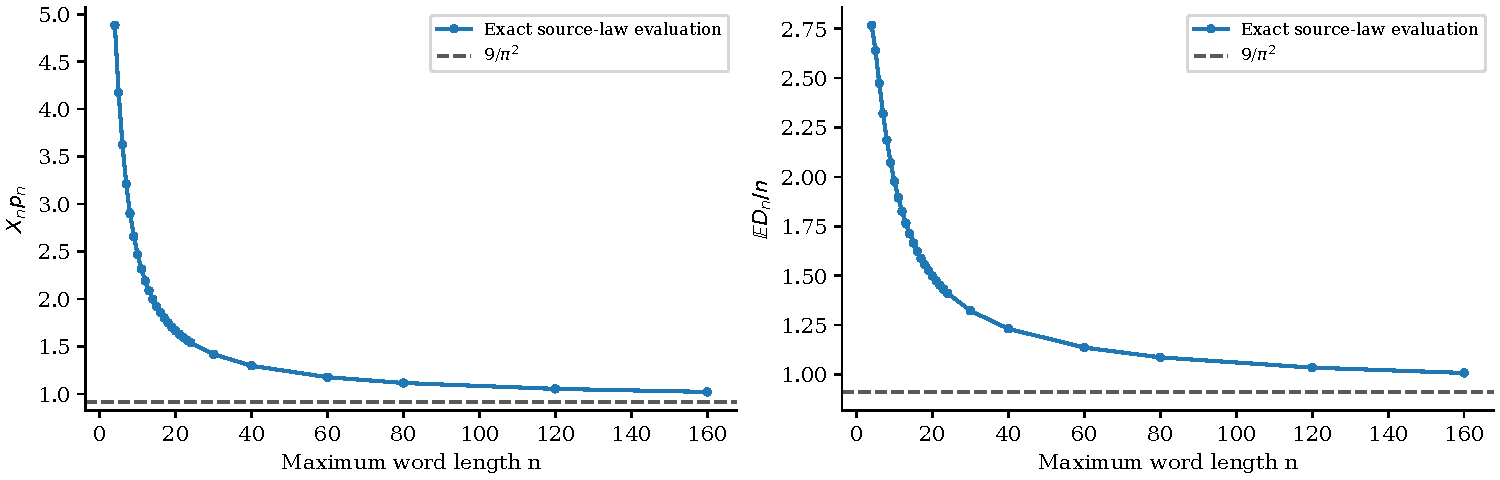
\includegraphics[width=\textwidth]{figures/source_scale.pdf}
\caption{Exact evaluation of the capped source law at $a_n=2-2/n$: $X_np_n$ (left) and $\EE D_n/n$ (right) against $n$, with the limit $9/\pi^2$. These are source-law values, not kinetic success probabilities.}\label{fig:source}
\end{figure}

\subsection{Proof of the \texorpdfstring{$\Theta$}{Theta} law and the ratio limit}
Let $V(n)\ge10^{60}(n+1)^2$. Then $V(n)\ge2n/d$ and $cV(n)/n\ge3n$ for all $n\ge1$ (with $c=d^2/(4\cdot10^7)$, $10^{60}c\ge6\cdot10^{10}$), so $\delta_{n,V(n)}\le e^{-3n}$. By \eqref{eq:sourcelimits}, $p_n\ge e^{-2n}$ eventually, hence $\delta_{n,V(n)}/p_n\le e^{-n}\to0$. Since $q_{0,n}\to6/\pi^2$, the sandwiches \eqref{eq:sandwich}--\eqref{eq:jointsandwich} give, eventually,
\[
 \frac12\Bigl(\frac6{\pi^2}\Bigr)^6p_n\le\PP(\cF_{n,V(n)}\cap G_n)\le\PP(\cF_{n,V(n)})\le(C_k+1)p_n ,
\]
which is the first two statements of \eqref{eq:theta-law}, and $\frac1n\log\PP(\cF_{n,V(n)})\to-\log2$. Dividing $\PP_0(\cF_{n,V(n)})\le2\delta_{n,V(n)}$ by the lower bound proves \eqref{eq:ratio}. \qed

\subsection{The conditional conclusion}\label{sec:conditional}
\begin{corollary}\label{cor:conditional}
At $a=a_n$ and along $V(n)\ge10^{60}(n+1)^2$,
\[
 \PP(\cF_{n,V(n)}\mid G_n)=\frac{\PP(\cF_{n,V(n)}\cap G_n)}{P_n}=\Theta(p_n)\longrightarrow0 .
\]
\end{corollary}
\begin{proof}
The numerator is the joint probability, bounded on both sides by \eqref{eq:jointsandwich}; its lower bound comes from the witness event $E_n$, which is contained in $G_n$ because $\{r_*\}$ is a RAF on $E_n$, and not from any independence between output and RAF existence. The denominator $P_n$ is at most $1$ and tends to $\thetaq>0$ by Theorem~\ref{thm:main}\ref{it:exist}, so it lies eventually in $[\thetaq/2,1]$. Division gives the claim.
\end{proof}
Thus, in the same sampled network, structural autocatalysis is present with probability bounded away from zero while the specified productive operation is present with probability of order $1/X_n$, and conditioning on the former does not change the order of the latter. This is tied to the fixed feed, bounded coefficients, observable and window; it does not declare any RAF inactive.

\subsection{Proof of Corollary~\texorpdfstring{\ref{cor:environment}}{3.3}}\label{sec:envproof}
The lower bound \eqref{eq:envlower} restates \eqref{eq:conditional} and \eqref{eq:Eprob}: on $E_n\times\{\text{all marks}\}$, $\pi_{n,V}\ge K(\cS_{n,V})\ge1-24\delta_{n,V}$. The upper bound \eqref{eq:envupper} restates \eqref{eq:pointwiseupper}: $\{\pi_{n,V}>4\delta_{n,V}\}\subseteq H_k\times\{\text{all marks}\}$, of probability at most $C_kp_n(a)$. The disabled statement is Section~\ref{sec:upper}. For the last sentence, fix $\eta\in(0,1)$; along $V(n)$ both $24\delta$ and $4\delta$ are eventually below $\min(\eta,1-\eta)$, so $\{\pi\ge1-24\delta\}\subseteq\{\pi\ge\eta\}\subseteq\{\pi>4\delta\}$, and the same inclusions hold after intersecting with $E_n\subseteq G_n$ on the left and with $G_n$ on the right. \qed

\subsection{What the volume envelope buys}\label{sec:volume}
The envelope $10^{60}(n+1)^2$ is convenient for the joint statement. The finite theorem gives a smaller sufficient volume for a prescribed reliability: for $0<\eta<1$,
\begin{equation}\label{eq:volume}
 V\ \ge\ \max\Bigl\{\frac{2n}d,\ \frac nc\log\frac{24}\eta\Bigr\}\quad\Longrightarrow\quad
 \inf_{\omega\in E_n,\ m}K_{n,V,\omega,m}(\cS_{n,V})\ge1-\eta ,
\end{equation}
because the right side is exactly $24e^{-cV/n}\le\eta$. To make a noise term $Ce^{-cV/n}$ smaller than $\eta p_n$, replace $24/\eta$ by $C/(\eta p_n)$; since $\log(1/p_n)\sim n\log2$, a quadratic scale suffices to make molecular noise smaller than environmental rarity. Neither \eqref{eq:volume} nor the larger envelope is a necessary-volume statement. The constants $d,c$ come from the concentration inequalities of Appendix~\ref{app:noise} with the tolerances of \eqref{eq:allowances}, the smallest of which is $\rho/100$; they are sufficient proof bounds, not fitted or physically calibrated thresholds.

\begin{remark}[Independent complete trials]
Since $p_n\sim9/(\pi^2X_n)$, every probability in \eqref{eq:theta-law} is $\Theta(1/X_n)=\Theta(n/R_n)$. For independent complete trials, each resampling environment, marks and trajectory, the number of trials to the first productive one is geometric with mean $\Theta(X_n)$; with $m$ trials the success probability is $1-(1-P)^m$, which tends to $0$ when $m/X_n\to0$ and to $1$ when $m/X_n\to\infty$. Repeated runs in one fixed environment are not independent complete trials, and a $\Theta$ law gives no Poisson constant at $m\asymp X_n$. Exponential decay in $n$ is polynomial decay in the explicitly enumerated catalog size and is not a computational hardness statement.
\end{remark}

\section{Discussion}\label{sec:discussion}

\paragraph{What the separation says.}
Theorem~\ref{thm:main} compares, in one probability space, a structural certificate and a productive requirement. The certificate is present with limiting probability $\thetaq\in(0,1)$ and, when present, is typically small. The requirement, bounded mass plus a fixed positive export from food alone in a fixed window, has probability of order $1/X_n$, and its conditional probability given the certificate has the same order. Removing catalysis makes the requirement asymptotically impossible at the same scale, so the productive events that do occur are catalytic. The two probabilities differ because they measure different things: the certificate is insensitive to rates, concentrations and competition, whereas the productive event needs a catalyst--substrate incidence that is \emph{short} in the sense of Section~\ref{sec:upper}, and short incidences are rare under the sampler. The lower bound shows that one such incidence, with food that catalyzes nothing, already suffices in the presence of arbitrary further nonfood catalysis.

\paragraph{What it does not say.}
The theorem is stated for one sampler, one exponent sequence, one reactor with fixed coefficients, and one observable with fixed window and thresholds. It does not say that RAF theory is wrong, that RAFs are dynamically inert, or that productive chemistry is universally rare. The constants are explicit but enormous, in both directions: $C_k$ counts a catalog of length-$4\cdot10^8$ words, and the volume envelope contains $10^{60}$. The result is an asymptotic order statement with a logarithmic rate, not a calibrated transition. Remark~\ref{rem:notclaimed} records that nothing is claimed about the RAF size of typical productive environments. The reactor is an effective, unsaturated, well-mixed mass-action model; spatial structure, saturation, measured molecular energies and heredity are outside its scope.

\paragraph{Relation to the structural literature.}
Hordijk and Steel \cite{hordijk2016variable} introduced the capped power-law variant and reported by simulation that heterogeneous catalysis lowers the level of catalysis required for RAF emergence and changes RAF sizes. Part \ref{it:exist} and Remark~\ref{rem:universality} show that, at the level of the limiting existence probability at linear intensity, the capped-Zipf law at $a_n=2-2/n$ is governed by the same survival function as the uniform law of the companion paper \cite{criticalwindow2026}; what the tail changes is the fluctuation structure on the growing catalogue, which is exactly what the two-band construction of Section~\ref{sec:construction} exploits to keep certificates small. The minimum RAF question is computationally hard in general \cite{steel2019autocatalytic}; part \ref{it:size} is a probabilistic statement about a typical sampled network, with no algorithmic content.

\paragraph{Relation to the kinetic literature.}
Kinetic simulations of the binary polymer model go back to \cite{farmer1986autocatalytic}; stochastic small-number effects and incoming flux were studied in \cite{filisetti2011stochastic}, and resource focusing with food-only initiation in \cite{giri2012origin}. The evolvability critique of \cite{vasas2010lack} and the response of \cite{hordijk2014evolvability} concern selection between RAFs rather than the existence of production; the present theorem is a statement about one step earlier, whether a sampled RAF-containing network produces at all in a fixed window. The corrected growth function $\Phi$ belongs to the family of average Lyapunov and auxiliary functions used in permanence theory \cite{patel2018robust} and in bounding time averages \cite{tobasco2018optimal}; its inequalities are established directly for this model. The transfer from drifts to trajectories is proved from the marked jump kernel (Appendix~\ref{app:noise}) rather than through a fluid-limit theorem of the type surveyed in \cite{darling2008differential}, because the error must be controlled at the scale $e^{-cV/n}$ where it is used, uniformly over the environment.

\paragraph{Numerical illustration.}
Figure~\ref{fig:mechanism} shows the deterministic mass-action trajectory of one specified environment in the complete $n=4$ catalog (30 species, 68 channels), with all basal reactions at the coefficients \eqref{eq:parameters}, the feed, the dilution, the self-catalyzed ligation $r_*$, and four further nonfood catalytic assignments chosen explicitly so that $E_4$ holds. It is a mechanism illustration, not a sample from the source law and not a count-process simulation; the probability theorem is analytic. The stored DOP853 computation uses absolute tolerance $10^{-18}$ and compares relative tolerances $10^{-10}$ and $2\cdot10^{-12}$: the maximum discrepancy over the saved arrays is below $1.6\cdot10^{-8}$ and the total mass differs from $10$ by less than $8\cdot10^{-15}$. Enabled and disabled export over $(1,100]$ are approximately $162.69$ and $4.15\cdot10^{-5}$; export can exceed instantaneous mass because the reactor is continuously fed. These are numerical diagnostics, not rigorous integration certificates.

\begin{figure}[ht]\centering
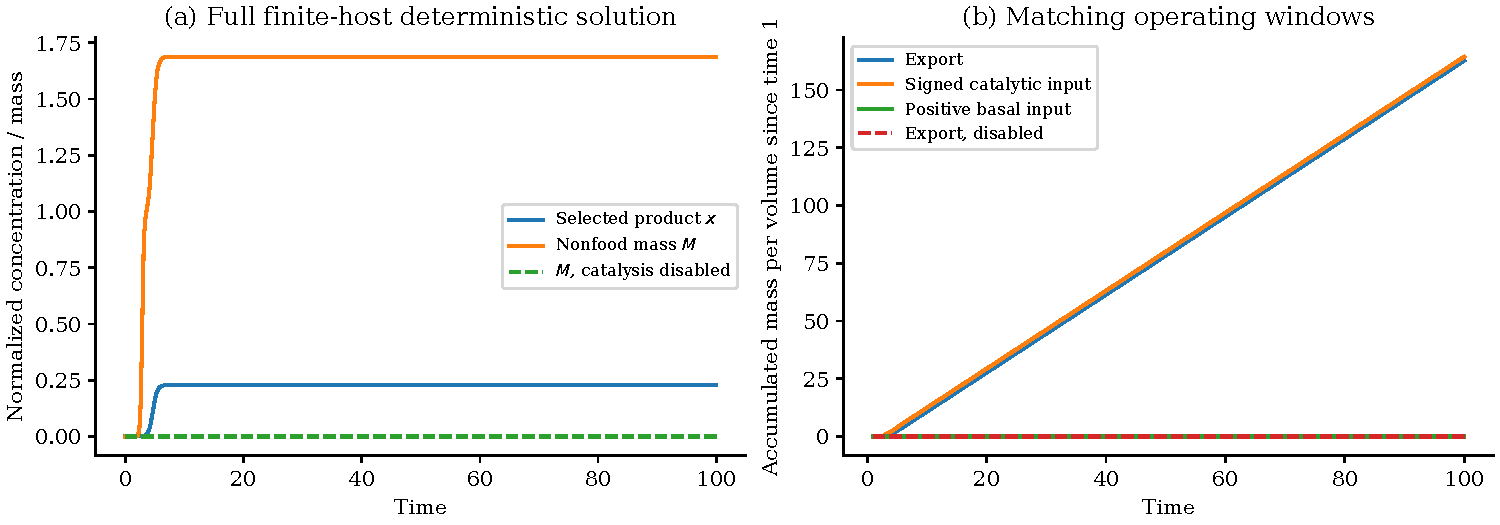
\includegraphics[width=\textwidth]{figures/mechanism.pdf}
\caption{A specified finite host at the theorem's kinetic parameters ($n=4$). Left: the selected product $x=x_{0011}$ and the total nonfood mass $M$, with the catalysis-disabled trajectory. Right: signed catalytic input, positive basal input and export, accumulated over $(1,t]$, with the disabled export. The disabled trajectory keeps the same basal rates and feeds.}\label{fig:mechanism}
\end{figure}

\paragraph{Further results left to a supplementary report.}
Three results proved in the same framework are omitted here because they concern different questions. A rare-event theorem attributes productive operation to one specified RAF at a much smaller volume $V=40+\lfloor\sqrt n\rfloor$, with a paid-path lower bound and a catalog upper bound giving the same logarithmic rate $-\log2$ but no uniform $\Theta$ law. A deterministic proposition shows that the mass-action trajectory of any environment in $E_n$ sustains a positive long-time mean catalytic input. A recurrence proposition shows that at any fixed finite volume the count process is positive recurrent and returns to the empty state, so that everlasting residence above a product floor is impossible; finite-window reliability as $V\to\infty$ and eventual loss as $t\to\infty$ at fixed $V$ are different limits and do not conflict.

\appendix

\section{The shifted growth inequality}\label{app:shift}
This appendix proves \eqref{eq:robust}. Put $\Dp(v)=(1-v)_+$ and $\eta=10^{-5}$. Let $a_u,a_w,a_x$ be the compensated coordinate errors, with $|a_u|,|a_w|\le\eta$, $|a_x|\le x/100$ and $C=C(M)\ge0$. Between jumps the corrected coordinates $u-a_u$, $w-a_w$, $x-a_x$ are absolutely continuous with derivatives equal to the coordinate drifts; across jumps the same holds because the jumps of a coordinate and of its compensated error coincide. Hence
\[
 \widetilde\Phi=\log(x-a_x)-4\Dp(u-a_u)^2-4\Dp(w-a_w)^2
\]
is absolutely continuous on any interval where $x$ is bounded away from zero; the squared positive part is continuously differentiable, including at its corner.

The elementary inequalities $\Dp(u-a_u)\le1+\eta$ and $\Dp(u)^2\le\Dp(u-a_u)^2+3\eta$, together with \eqref{eq:fooddrift}, give
\[
 8\Dp(u-a_u)\,b_u\ \ge\ 8\Dp(u-a_u)^2-46C-8(1+\eta)\eta(1+23C),
\]
where $\Dp(u-a_u)u\le(1+\eta)^2/4$ bounds the depletion term; the unshifted coefficient is $46$ and the explicit error term covers the perturbation. The same holds for $w$. Positivity of the basal term in \eqref{eq:productdrift} and $|a_x|\le x/100$ give
\[
 \frac{b_x}{x-a_x}\ \ge\ 0.99\,(4uw)-1.02\,(1+25C).
\]
For $u,w\ge0$,
\[
 0.99\,(4uw)+8\Dp(u)^2+8\Dp(w)^2\ \ge\ 2.97 ,
\]
as one checks by minimizing on $[0,1]^2$ and on its boundary; replacing a coordinate larger than $1$ by $1$ cannot increase the expression. Combining the three estimates, the constant term exceeds $1.9$ and the coefficient of $-C$ is smaller than $120$, which is \eqref{eq:robust}.

On the good event $x\ge\rho$ and $L\le11$, so $x-a_x\ge\rho/2$ and $x-a_x\le3$, and the total possible increase of $\widetilde\Phi$ on $[1,100]$ is less than
\[
 \log(6/\rho)+8(1+\eta)^2<54 ;
\]
for instance $e>65/24$ and $(65/24)^{45}>18\cdot10^{18}=6/\rho$ verify the logarithm without transcendental evaluation. Integration of \eqref{eq:robust} over $[1,100]$ gives \eqref{eq:integral}. No logarithm of a jump process is treated as a drift-only quantity: the logarithm is applied to the continuous compensated coordinate.

\section{Stopped kernel bounds and physical time}\label{app:noise}
We give the concentration argument behind $\delta_{n,V}$, including the final incomplete holding interval. Stop at the first exit from $\{L\le11\}$ or at time $T=101$. On this region the total jump rate is at most $24000V$ by \eqref{eq:hazard}. Each concentration coordinate jumps by at most $2/V$, with quadratic-variation rate at most $96000/V$. For the nonfood mass and for the export and positive-input rewards, an internal jump has magnitude at most $4/V$, an outflow jump at most $n/V$, and the outflow quadratic-variation contribution is bounded using $V^{-2}\sum_x\ell(x)^2N_x\le nL/V$; so the reward quadratic-variation rate is at most $(384000+11n)/V\le96011n/V$ for $n\ge4$.

\emph{Marked-kernel supermartingale.} In a state with channel rates $\lambda_j$ and total rate $q$, the next waiting time and mark have density $\lambda_je^{-qs}\,ds$. If $r_j$ are bounded reward increments, $\mu=\sum_j\lambda_jr_j$ and $Q\ge\sum_j\lambda_jr_j^2$, then
\[
 \sum_j\lambda_j\bigl(e^{\vartheta r_j}-1\bigr)\le\vartheta\mu+\vartheta^2Q\qquad(|\vartheta r_j|\le1),
\]
by $e^v\le1+v+v^2$ on $[-1,1]$. Multiplied by the compensating waiting-time factor, the exponential of $\vartheta\times$(reward minus compensator) minus $\vartheta^2\times$(integrated $Q$) is a nonnegative supermartingale along the jump chain. At a deterministic endpoint the no-jump survival term $e^{-qs}$ is included, so the compensator contains the elapsed part of the last holding interval; conditioning on completion of that interval would change the law and is not used.

\emph{Maximal inequality.} Stop the supermartingale at the first threshold crossing, apply the expectation bound, and pass from finitely many jumps to the full stopped path by monotone limits. Applying both signs of $\vartheta$ and optimizing within the admissible range gives, for a positive parameter $d$,
\begin{align*}
 \PP\bigl(\sup|A_{\rm reward}|>d+n/V\bigr)&\le2\exp\Bigl\{-\frac{d^2V}{4n(96011T+d)}\Bigr\},\\
 \PP\bigl(\sup|A_{\rm coordinate}|>d+2/V\bigr)&\le2\exp\Bigl\{-\frac{d^2V}{4(96000T+2d)}\Bigr\}.
\end{align*}
The added jump allowances permit one crossing jump and interpolation at physical-time endpoints. Rewards are frozen after the first mass exit and not restarted. The bounds need neither independent coordinates nor independent successive rewards; they hold conditionally on any environment, marks and history.

\emph{Constants.} With $d$ and $c$ from \eqref{eq:constants} and $T=101$, $\frac{d^2}{4n(96011\cdot101+d)}\ge\frac{c}{n}$ and $\frac{d^2}{4(96000\cdot101+2d)}\ge\frac cn$, so each two-sided failure probability is at most $2\delta_{n,V}$. For $V\ge2n/d$ the allowances $d+n/V\le\frac32d$ and $d+2/V\le\frac54d$ (using $n\ge4$) are smaller than every tolerance in \eqref{eq:allowances}, the smallest being $\rho/100=2d$. There are twelve applications: nonfood mass, six food coordinates for mass control, the two food coordinates $u,w$ at the tighter startup tolerance, the product $x$, the export, and the positive basal input; their union costs at most $24\delta_{n,V}$. The upper bound uses two reward applications ($4\delta_{n,V}$) and the disabled bound one ($2\delta_{n,V}$).

\emph{Mass localization.} The compensated total-mass error is bounded by $|A_L|\le\frac18+\sum_{f\in F}\ell(f)\frac1{80}=\frac14$. The linear comparison \eqref{eq:scalar} applied to $\cG L=10-L$, $L(0)=10$, gives $L\le10.5$ up to the putative first exit, and the crossing-jump convention excludes an exit through $11$ on the good event. The food and product comparisons of Section~\ref{sec:transfer} are therefore valid throughout $[0,T]$.

All events are measurable in the jump representation, and nonexplosion with almost surely positive holding times identifies them with their physical-time counterparts. Integrating the finite source law, the marks and the jump law produces the probabilities in Theorem~\ref{thm:main}.

\section{Structural proof details}\label{app:structural}
This appendix supplies the finite identities, the independent-closure facts, the degree-band coupling, the target estimate and the assembly used in Section~\ref{sec:structural}. Throughout $a=a_n$.

\subsection{Finite source weights and local convergence}\label{app:finite}
For $A\subseteq\RR_n$ the one-row probability $\PP(C_x=A)$ is $\mu_{a,R_n}(|A|)/\binom{R_n}{|A|}$, and the configuration weight is \eqref{eq:weight}; normalization follows by grouping subsets by cardinality. For $s$ distinct channels the conditional one-row miss probability given $D_x=D$ is $\binom{R_n-s}{D}/\binom{R_n}{D}$, zero when $D>R_n-s$; the inclusion probabilities of one and two prescribed channels are $\EE D_n/R_n$ and $\EE[D_n(D_n-1)]/[R_n(R_n-1)]$, which give \eqref{eq:bonf}. The second factorial moment is at most the second moment and $R_n/(R_n-1)\to1$, so its scaled contribution vanishes by Lemma~\ref{lem:moments}. For disjoint finite $S,C$ the identity
\[
 \ind\{S\subseteq O,\ C\cap O=\varnothing\}=\sum_{T\subseteq S}(-1)^{|T|}\ind\{(T\cup C)\cap O=\varnothing\}
\]
holds for every set $O$, by expanding $\prod_{r\in S}(1-\ind\{r\notin O\})\prod_{r\in C}\ind\{r\notin O\}$; multiplying by \eqref{eq:weight} and summing needs no independence within a row. The embedding of $\RR_N$ into $\RR_n$ preserves product word and split position, hence all cardinalities, which proves Proposition~\ref{prop:catalogue}.

\subsection{Independent closure: records, nuclei, continuity}\label{app:iid}
\emph{Survival generates every target.} For any cap $B\ge2$, induction on a reversible derivation gives the alternative: the derivation fits inside cap $B$, or some accessible word $w$ has $\ell(w)>B$ and a derivation entirely inside cap $\ell(w)$ (at a ligation leaving $B$ the product is such a word; a cleavage inherits a record from its input). So survival supplies record words beyond every cap. Fix a target $v=v_1\cdots v_\ell$. Given a record $w$, the sequence $w\to wv_1\to\cdots\to wv$, $wv\to w+v$ uses food letters and at most $\ell+1$ channels, all with products longer than $w$, whose coordinates lie outside the $\sigma$-algebra of channels up to length $\ell(w)$; their joint openness has probability at least $q^{\ell+1}$. Fix a cylinder $A$ determined by a cap $B$ and partition the occurrence of a longer record into disjoint first-record atoms, each determined by the coordinates up to its own record length; on each atom the displayed support is fresh. Summing gives, for $H_v=\{\text{survival and }v\text{ missing}\}$,
\begin{equation}\label{eq:deficit}
 \PP(H_v\cap A)\le(1-q^{\ell+1})\PP(A)
\end{equation}
for every cylinder $A$. If $\PP(H_v)>0$, approximating its indicator by the increasing finite-coordinate $\sigma$-algebras would produce cylinders with conditional density arbitrarily close to one, contradicting \eqref{eq:deficit}. Hence $\PP(H_v)=0$, and a countable union over $v$ shows that survival implies complete closure almost surely.

\emph{Finite witnesses and continuity above one half.} Let $F_m(q)$ be the event that the closure generates all words of length at most $m$; it is the increasing union over $N$ of the events $F_{m,N}(q)$ that all these derivations exist inside cap $N$, so $\PP(F_{m,N}(q))\uparrow\PP(F_m(q))\ge\theta(q)$. If every word longer than $m$ has an open split, $F_m(q)$ implies complete closure by induction on length; the probability that the split condition fails is at most $\tau_m(q)$ in \eqref{eq:seedtail}, a union bound valid even when the finite witness uses channels beyond length $m$. Hence $\PP(F_m(q))\le\theta(q)+\tau_m(q)$. For positivity of $\theta$, require all channels through a fixed $m$ open; channels with longer products are independent of this, and the sum of their word-level failure probabilities is finite, so the infinite product of success probabilities is positive and their intersection implies survival. For left continuity at $q>1/2$: fix $q_0\in(1/2,q)$, choose $m$ with $\tau_m(q_0)<\eta$ and $N$ with $\PP(F_{m,N}(q))>\theta(q)-\eta$; the finite-cap probability is a polynomial in the openness, so for $q'\uparrow q$ it eventually exceeds $\theta(q)-2\eta$, and then $\theta(q')\ge\PP(F_{m,N}(q'))-\tau_m(q')>\theta(q)-3\eta$; monotonicity gives the other inequality. For right continuity, survival is the decreasing intersection of the fixed-boundary escape events, each determined by a finite catalogue with continuous probability, whose probabilities bound $\theta$ from above. This suffices at $q_*>1/2$.

\subsection{Degree bands and the source coupling}\label{app:degree}
With $h_n,L_n,k_n,d_0,d_1,d_2,\eps_n$ as in \eqref{eq:budget} and \eqref{eq:bands}, eventually $d_0\le d_1<d_2<R_n$. Put $Y_L=D_n\ind\{d_0\le D_n<d_1\}$ and $Y_H=D_n\ind\{d_1\le D_n<d_2\}$; both intervals lie below the cap atom. Integral comparison for $(d+1)^{-a_n}d$, with negligible normalized endpoint errors, gives
\begin{equation}\label{eq:bandmeans}
 \frac{\EE Y_L}n\longrightarrow\frac3{2\zeta(2)}=\Lambda,\qquad \frac{\EE Y_H}{h_n}\longrightarrow\frac{19\log2}{5\zeta(2)} .
\end{equation}
For the first, $\log d_0/n\to0$, $\log d_1/n\to\log2$, and the primitive of $x^{-1+2/n}$ is $\frac n2x^{2/n}$. For the second, with $u=\log x/n$ the integral is $n\int e^{2u}du$ over an interval of width $[h_n-\lfloor h_n/20\rfloor]\log2/n$ near $u=\log2$, whose integrand tends uniformly to $4$, giving $4\cdot\frac{19}{20}\log2$ after division by $h_n$.

For either band variable $0\le Y\le U$, independence of degrees gives $\operatorname{Var}(\sum_xY_x)\le X_n\EE Y^2\le X_nU\EE Y$ with $U\le X_n$ eventually, so a relative downward deviation $\delta$ has probability at most $1/(\delta^2\EE Y)$; both band means diverge, so the relative deficits vanish. For the low union, conditional openness is
\[
 q_L(d)=1-\prod_{x:\,d_0\le d_x<d_1}\Bigl(1-\frac{(1-\eps_n)d_x}{R_n}\Bigr)\ \ge\ 1-\exp\Bigl(-\frac{1-\eps_n}{R_n}\sum_xY_{L,x}\Bigr),
\]
which by \eqref{eq:bandmeans} and $R_n/(nX_n)\to1$ is at least $1-e^{-t}$ with probability tending to one, for each $t<\Lambda$. For the high union, with retention $19/20$ and relative deficit $1/50$, the normalized exponential intensity has lower limit
\begin{equation}\label{eq:margin}
 \frac{49}{50}\cdot\frac{19}{20}\cdot\frac{19\log2}{5\zeta(2)}>1.47>\frac{29}{20},
\end{equation}
and since $1-e^{-z}\sim z$ this gives the floor $\pi_n=\frac{29}{20}n^{-1/4}$ eventually, outside a vanishing degree exception. The strict margins in \eqref{eq:margin} are specific to $a_n=2-2/n$.

\emph{Exact row marginals.} Conditional on the degrees, generate independent auxiliary Bernoulli subsets $A_x$ with the stated per-channel probabilities. A binomial Chernoff bound gives $\PP(|A_x|>d_x\mid d)\le e^{-\eps_n^2d_x/4}$ for low rows, and eventually $\eps_n\le1/20$ covers the high rows. On $|A_x|\le d_x$ complete $A_x$ to a uniform $d_x$-subset; on overflow choose a uniform $d_x$-subset independently. The result is uniform by invariance under channel permutations, and on no overflow every auxiliary incidence is a source incidence. Doing this independently across rows and integrating the exact degree law gives the coupling, with total overflow probability at most $X_ne^{-\eps_n^2d_0/4}\le e^{-n}$ eventually; inactive rows cost nothing. This is an increasing-event transfer with an explicit exceptional event, not a stochastic domination claim.

\emph{Number and length of labels.} Since $\EE D_n\le2n$ eventually, Markov's inequality gives $\PP(\#\{x:D_x\ge d_1\}\ge n^32^{h_n})\le X_n\EE D_n/(d_1n^32^{h_n})\le4/n^2$. For a length threshold $s$ and degree threshold $d$, a union bound and Markov's inequality give $\PP(\exists x:\ell(x)<s,\ D_x\ge d)\le2^s\EE D_n/d$; at $(s,d)=(n-2h_n,d_1)$ and $(k_n-h_n,d_0)$ these are $O(n2^{-h_n})$. They hold before any owner is selected, and every selected low label has degree at least $d_0$, so the second exclusion covers the whole adaptive selection. This proves \eqref{eq:owners}.

\subsection{The uniform bounded target estimate}\label{app:target}
Let $w$ be a fixed word of length $\ell$ and let the independent field have openness $p$. Work with the distinct nonempty substrings of $w$, ordered by length, with all substrings of length at most $L$ available. For each distinct longer product word $u$ expose its full row of split-position bits; rows of different product words are independent, and repeated occurrences of a substring use the same row and are never counted as independent trials.

Call $u$ \emph{cut-dense} for the current known set if at most $\ell(u)/8$ of its proper prefix cuts have a missing prefix and at most $\ell(u)/8$ have a missing suffix. For $\ell(u)\ge4$, cut density gives at least $\ell(u)/2$ usable splits, so conditionally on the history of shorter words the probability that $u$ is not generated is at most $e^{-p\ell(u)/2}$. If cut density fails somewhere after the exploration, take a shortest failing word $u$; one side has more than $\ell(u)/8$ missing proper parts, with cut-index set $J$. Each such part has length greater than $L$, is cut-dense by minimality, and is a distinct word (for a fixed side, different cut indices give different lengths). For fixed $u$, side and $J$, summing over exposure histories, each selected part fails while cut-dense and charges at least $p/2$ times its length through its fresh row; iterated conditional expectation bounds the joint probability by $\exp(-\frac p2\sum_{i\in J}\ell(u_i))\le\exp(-pL\ell(u)/16)$. The density predicates refer to the final known set, but the shorter parts of each word are settled at its exposure, so the length ordering makes the charging valid. There are at most $2^{\ell(u)}$ sets $J$; if $pL\ge32\log2$ and $\ell(u)\ge L$ then $2^{\ell(u)}e^{-pL\ell(u)/16}\le e^{-pL^2/32}$. With two sides and at most $\ell^2$ distinct substrings, any density failure has probability at most $2\ell^2e^{-pL^2/32}$, and in its absence the failure of $w$ itself costs at most $e^{-p\ell/2}$. This is \eqref{eq:target}.

On success, choose one successful split per needed product and trace a derivation of $w$ to leaves in the nucleus; the tree has at most $\ell$ leaves (nonempty pieces partitioning $w$), hence at most $\ell-1$ internal nodes and at most $\ell-1$ distinct added channels. If a base support $S_0(H)$, possibly depending on the high field $H$, generates the nucleus, then raw exploration success supplies a bounded additional support in $H$ regardless of that dependence; the guarded event that the base generates the nucleus but no bounded support exists is contained in the raw failure event. For the selected low targets, condition on the degrees and the low rows first, fixing targets and base; the high field then has the independent law just analysed, and a union bound over the fixed target list followed by averaging is legitimate.

\subsection{Assembly and reversible trimming}\label{app:assembly}
Fix an admissible low openness $q\in(1/2,q_*)$ and $t<\Lambda$ with $q\le1-e^{-t}$. Choose $m$ with $\tau_m(q)<\eta$ and a seed cap $N$ capturing mass greater than a chosen $c<\theta(q)$. Retain all channels of the seed witness inside cap $N$ (at most $R_N$), require an open split for every word of length $m+1,\dots,L_n$ and retain one such split; the extension loss is bounded by $\tau_m(q)$ uniformly in $L_n$. Select a low-row catalyst for each retained channel; support and label list have size at most $R_N+2^{L_n+1}$. The high target set is $W_H$. The deterministic bounds and the guarded target estimates give a good event on which the union of the base and all target derivations has size at most $b_N(n)$ in \eqref{eq:seedbudget}. The loss from seed-and-extension mass to an actual source RAF is at most the sum of five vanishing terms: (1) high-target inadmissibility (too many high labels or a too-short high label); (2) a too-short active low label; (3) guarded failure of a bounded high-label derivation, including the high-openness exception; (4) guarded failure of a bounded selected-low-label derivation, including the same exception; (5) overflow in the Bernoulli-row coupling. Counting an openness exception in both envelopes is harmless, and no factorization of seed and target success is used: an indicator inequality and summation suffice.

Let $S$ be the assembled support; every channel of $S$ has a catalyst in $\cl_F(S)$. Let $T\subseteq S$ consist of the channels at least one direction of which becomes enabled at some finite stage of the closure. Induction on closure stages gives $\cl_F(T)=\cl_F(S)$, since every productive step of $S$ uses a channel retained in $T$. For a channel in $T$ its enabled direction places both sides in the closure, and its catalyst remains generated because the closure is preserved. A word of length three is generated, so $T\ne\varnothing$; hence $T$ is a RAF with $|T|\le|S|$. For every $r<\theta(q)$ choose the seed and extension margins before letting $n\to\infty$; the five errors and the low-openness exception vanish, giving $P_n(b_N(n))>r$ eventually. Continuity of $\theta$ and $q\uparrow q_*$ supply every $r<\thetaq$, which is Proposition~\ref{prop:lower}.

\subsection{First-exit adapters}\label{app:exit}
The source-open set $O_n$ contains every RAF support, and monotonicity of reversible closure embeds all internally generated catalysts into $\cl_F(O_n)$. A first food-enabled channel of a nonempty RAF has product length at most four, and the whole catalogue through length four has $R_4=68$ channels. For fixed $K\ge2$, the first productive step escaping length $K$ cannot be a cleavage; its two ligation inputs have length at most $K$ and its product length lies in $(K,2K]$, and induction on the preceding derivation gives exact equality of the escape event with its restriction to cap $2K$ for $n\ge2K$, product words and split positions embedding literally. If escape fails but a RAF exists, a food-enabled channel has an internally generated catalyst of length at most $K$; each specified pair has source probability exactly $\EE D_n/R_n$, giving Lemma~\ref{lem:upper}. The argument uses neither a bound on the number of RAF witnesses nor independent catalysis by accessible molecules.

\section{Formal verification and reproducibility}\label{app:formal}
The formal developments use Lean~4 (toolchain \texttt{leanprover/lean4:v4.30.0}) with the repository's frozen Mathlib manifest (Mathlib commit \texttt{c5ea00351c28e24afc9f0f84379aa41082b1188f}; manifest SHA-256 \texttt{a8df0b60\ldots}). Strict verification compiles the local import closure with warnings treated as errors, rejects \texttt{sorry}, and audits the axioms of the selected declarations; every selected declaration depends only on \texttt{Classical.choice}, \texttt{Quot.sound} and \texttt{propext}. No stochastic estimate is added as an axiom. Verification receipts record source hashes, dependency hashes, commands and axiom audits; their proof-file hashes are quoted below by their first sixteen hexadecimal digits.

\subsection{Concordance}
{\raggedright The structural development is the namespace \lean{PowerLawSmallRAF}; the reactor development is \lean{RandomViability}, which imports it. In the reactor development the source law is \lean{sourcePowerLawConfigWeight}, the RAF event is \lean{anySourceRAF} (existence of a reversible RAF for \lean{binaryPolymerCRS n 2} with the sampled catalysis), the productive event is \lean{physicalOutputEvent} (mass at most $11V$ through time $100$ and windowed export reward above $1/10$ on $(1,100]$), the joint probability is \lean{outputJointProbability} (source average, mark average and trajectory law), the incidence is \lean{productiveSourceIncidence} $=p_n$, the noise rate is \lean{markedNoiseRate} $=c$, and the volume envelope is \lean{collectiveMinimalVolume} $=10^{60}(n+1)^2$.\par}

\begingroup\small
\setlength{\tabcolsep}{4pt}
\begin{longtable}{@{}>{\raggedright\arraybackslash}p{.30\textwidth}>{\raggedright\arraybackslash}p{.66\textwidth}@{}}
\toprule Statement in this paper & Lean declaration (module; receipt hash prefix)\\\midrule\endhead
Lemma~\ref{lem:moments} & \lean{sourceExactCriticalFirstMoment_scaled_tendsto}, \lean{sourceExactCriticalSecondMoment_scaled_tendsto_zero} (\lean{SourceCriticalSecondMoment.lean})\\[3pt]
Proposition~\ref{prop:catalogue} & \lean{sourceFiniteCap_event_tendsto} (\lean{SourceFiniteCapLimit.lean})\\[3pt]
Nucleus and survival (App.~\ref{app:iid}) & \lean{fixed_seed_captures_survival_with_small_extension_error} (\lean{FixedSeedSurvivalApproximation.lean})\\[3pt]
Target estimate \eqref{eq:target} & \lean{finite_ligation_target_failure_bound} (\lean{FiniteLigationTarget.lean}); \lean{source_bounded_target_failure_bound} (\lean{BoundedTargetProbability.lean})\\[3pt]
Source coupling (App.~\ref{app:degree}) & \lean{sourceFiniteSeedMass_eventually_le_source} (\lean{FiniteSeedSourceProbability.lean})\\[3pt]
Proposition~\ref{prop:lower} & \lean{source_subexponential_RAF_endpoint_lower} (\lean{SourceCriticalEndpoint.lean})\\[3pt]
Lemma~\ref{lem:upper}, \eqref{eq:limsup} & \lean{sourceFullRAFProbability_le_escape_add_seed} (\lean{SourceEscapeProbability.lean}); \lean{sourceEscapeProbability_tendsto} (\lean{SourceEscapeLimit.lean}); \lean{source_RAF_survival_upper} (\lean{SourceRAFSurvivalUpper.lean})\\[3pt]
Theorem~\ref{thm:main}\ref{it:exist}, limit & \lean{PowerLawSmallRAF.source_RAF_probability_tendsto} (\lean{Main.lean}; \texttt{425914e5b768a3d1})\\[3pt]
Theorem~\ref{thm:main}\ref{it:size}, cutoff limits & \lean{source_subexponential_cutoff_probability_tendsto}, \lean{source_conditional_minimum_subexponential} (\lean{Main.lean})\\[3pt]
Theorem~\ref{thm:main}\ref{it:size}, explicit $B_n$ and tails & \lean{sourcePublicationBudget_subexponential}, \lean{source_publication_cutoff_probability_tendsto}, \lean{source_conditional_publication_cutoff_tendsto}, \lean{source_large_minimum_exception_probability_tendsto_zero}, \lean{source_conditional_exponential_rate_tail_tendsto_zero} (\lean{PowerLawSmallRAF/PublicationCorollaries.lean}; \texttt{fb71101d4a92c251})\\[3pt]
Capacity bound, Lemma~\ref{lem:capacity} & \lean{catalyticFoodEnvelope_mass_bound} (\lean{FoodUptake.lean}); \lean{positive_catalytic_drift_small} (\lean{MarkedCatalyticInput.lean})\\[3pt]
Startup floors, Section~\ref{sec:transfer} & \lean{physical_food_prefix_floor} (\lean{PhysicalFoodStartup.lean}); \lean{physical_product_interval_floor} (\lean{PhysicalProductStartup.lean})\\[3pt]
Output event; finite success inclusion; pointwise upper and disabled bounds & \lean{physicalOutputEvent}, \lean{finite_success_implies_output} (\lean{PhysicalOutputEvent.lean}; \texttt{223f4f297ca30db7}); \lean{physical_collective_upper_without_short_incidence} (\lean{MarkedCatalyticUpper.lean}); \lean{PhysicalOutputProbability.lean} (\texttt{07e443e1d91390dc})\\[3pt]
Finite sandwiches \eqref{eq:sandwich}--\eqref{eq:jointsandwich} & \lean{RandomViability.averaged_output_bounds} (\lean{SourceOutputProbability.lean}; \texttt{91502845f4191378})\\[3pt]
Disabled finite bound & \lean{RandomViability.averaged_output_disabled_bound} (same module)\\[3pt]
$\Theta$ law \eqref{eq:theta-law}, first two & \lean{RandomViability.label_free_output_theta}, \lean{RandomViability.output_and_some_raf_theta} (\lean{RandomViability/PublicationCorollaries.lean}; \texttt{1d10e1359bba5302}); \lean{output_joint_probability_theta} (\lean{OutputJointLimit.lean}; \texttt{5d333feb48191ce3})\\[3pt]
Ratio limit \eqref{eq:ratio} & \lean{RandomViability.disabled_enabled_output_ratio}\\[3pt]
Corollary~\ref{cor:conditional} & \lean{RandomViability.output_conditioned_on_raf_theta} (\lean{PublicationStructure.lean}; \texttt{7126ee713efed312}), which divides \lean{output_and_some_raf_theta} by \lean{source_raf_probability_positive}, itself derived from \lean{source_subexponential_RAF_endpoint_lower}\\[3pt]
$\EE D_n/n\to9/\pi^2$ & \lean{RandomViability.mean_degree_per_length_limit} (\lean{PublicationStructure.lean})\\[3pt]
Finite reliability \eqref{eq:volume} & \lean{RandomViability.noise_error_below_tolerance}, composed with \eqref{eq:conditional}\\[3pt]
Corollary~\ref{cor:environment}; $0<\thetaq<1$ upper bound; $M_n$ interpretation; independent-trial remark & Conventional consequences of the verified statements, proved in the text; not separate Lean exports\\
\bottomrule
\end{longtable}\endgroup

The receipt for \lean{PublicationStructure.lean} is the publication entry point for the productive half: its strict run compiled the whole import closure, including the structural development, in one pass. The structural terminal receipt covers the four root declarations of \lean{Main.lean}; the corollary receipt covers the five explicit-cutoff statements. A source audit compared the current bytes of every file in both closures ($566$ distinct local sources for the reactor closure; $365$ for the structural closure) with the hashes recorded in the receipts.

\subsection{Scope of the formalization}
The Lean statements are event-level: the minimum $M_n$ is not a formal random variable, and the cutoff theorems are stated as convergence of $P_n(\lfloor2^{bn}\rfloor)$ and of the conditional ratio; their reading as statements about $\log M_n/n$ is the elementary interpretation on the finite configuration space. The productive theorems are stated for the averaged probability $\PP(\cF_{n,V})$ and for the pointwise upper bound outside the short-incidence event; the environment-level Corollary~\ref{cor:environment} combines them in prose. The catalog constant $C_k$ appears in Lean as \lean{collectiveSourceUpperConstant}. The results left to the supplementary report (attribution at small volume, deterministic sustained mean, finite-copy recurrence) are not used anywhere in this paper.

\subsection{Reproduction}
The manuscript source, bibliography, figure generator and figure data accompany the paper. The figure generator fixes the kinetic-mark seed and the four extra catalytic assignments of the $n=4$ host, checks mass conservation, compares two integration tolerances, and evaluates the source law with 100-digit Hurwitz-zeta arithmetic; it performs no Monte Carlo estimate of any rare event. Strict verification of the terminal declarations is run through the repository's verification bridge, which sets the Lean working directory to the frozen Mathlib project and enables warnings-as-errors; the commands are recorded with the receipts.

\bibliographystyle{plainnat}
\bibliography{refs}
\end{document}
